%!TeX program = xelatex

%
% Ogni volta che aggiungi font esegui:  D:\Program Files\MiKTeX 2.9\miktex\bin\x64> miktex-fc-cache -f
% Per aggiornare la cache (e metti anche xelatex.exe run as administrator)
%
% ============================================================================ %
%	PACKAGES E CONFIGURAZIONE BASE DOCUMENTO                                   %
% ============================================================================ %
\documentclass[
fontsize=11pt, % Base font size
twoside=true, % Use different layouts for even and odd pages (in particular, if twoside=true, the margin column will be always on the outside)
%open=any, % If twoside=true, uncomment this to force new chapters to start on any page, not only on right (odd) pages
%chapterprefix=true, % Uncomment to use the word "Chapter" before chapter numbers everywhere they appear
%chapterentrydots=true, % Uncomment to output dots from the chapter name to the page number in the table of contents
numbers=noenddot, % Comment to output dots after chapter numbers; the most common values for this option are: enddot, noenddot and auto (see the KOMAScript documentation for an in-depth explanation)
%draft=true, % If uncommented, rulers will be added in the header and footer
%overfullrule=true, % If uncommented, overly long lines will be marked by a black box; useful for correcting spacing problems
]{kao/kaobook}


% ============================================================================ %
% 								   METADATA                                    %
% ============================================================================ %
\def\VERSION{0.2} %VERSIONE DEL DOCUMENTO 

% ============================================================================ %
%                        PACKAGE BASE UTILIZZATI                               %
% ============================================================================ %
% Package di configurazione/stile/proprietà
\usepackage[english, italian]{babel}	      % Lingua principale del documento.
\usepackage[italian=quotes]{csquotes}	      % Italian quotes (virgolette)

% Package di utility/funzionalità
\usepackage{import}					          % Per importare tex esternamente

% Package di testing e debugging
\usepackage{blindtext}
%\usepackage{showframe} % Uncomment to show boxes around the text area, margin, header and footer
%\usepackage{showlabels} % Uncomment to output the content of \label commands to the document where they are used

% Load the bibliography package
\usepackage[backend=bibtex]{biblatex} 
\usepackage{kao/styles/kaobiblio}
\addbibresource{relazioneCG.bib} % Bibliography file

% Load mathematical packages for theorems and related environments.
\usepackage{kao/styles/mdftheorems}

% ============================================================================ %
%                                   INPUTS                                     %
% ============================================================================ %
% ============================================================================ %
%                             PACKAGE UTILIZZATI                               %
% ============================================================================ %
% Package di configurazione/stile/proprietà

% Package di utility/funzionalità
\usepackage{amssymb}						  % per \varnothing
\usepackage{amsmath}
\usepackage{relsize}                          % Per scalare in percentuale la dimensione dei font.     
\usepackage{subcaption}                       % Per avere subfigure e subcaption           
\usepackage{longtable}
\usepackage{multirow}                         % Per unire più row
\usepackage{hhline}                           %per line che si vedono --- replace \cline{2-4} by \hhline{~|-|-|-|}. The
%\usepackage[linesnumbered,ruled]{algorithm2e}

% Package grafici
\usepackage{siunitx}                          % Per formattare automaticamente i numeri nel testo \num{.}
                                              % aggiunge un tipo di colonna colonna S alle tabelle
\usepackage{lettrine}

\usepackage{multicol}                         %Per itemize/liste su più colonne 
                                              
			%Input dei package PRINCIPALI usati
% ============================================================================ %
%                             PACKAGE UTILIZZATI                               %
% ============================================================================ %
\usepackage{titlesec}					% Per la modifica dei titoli delle sezioni
\usepackage{tikz}
\usetikzlibrary{positioning,calc,shapes}
\usepackage{calc}						% Per effettuare calcoli
\import{inputs/}{defined-colors}
\captionsetup[table]{position=bottom}

% --------------------------------------------------------------------------- %
%	Utility                 				                                  %
% --------------------------------------------------------------------------- %
% Per ottenere i nomi di chap, section, subsection e subsubsection attuali. 
\let\Chaptermark\chaptermark
\def\chaptermark#1{\def\Chaptername{#1}\Chaptermark{#1}}
\let\Sectionmark\sectionmark
\def\sectionmark#1{\def\Sectionname{#1}\Sectionmark{#1}}
\let\Subsectionmark\subsectionmark
\def\subsectionmark#1{\def\Subsectionname{#1}\Subsectionmark{#1}}
\let\Subsubsectionmark\subsubsectionmark
\def\subsubsectionmark#1{\def\Subsubsectionname{#1}\Subsubsectionmark{#1}}


% --------------------------------------------------------------------------- %
%	Personalizzazione: Fonts				                                  %
% --------------------------------------------------------------------------- %
\iftrue
	%XeLaTeX packages per font
	\usepackage{xltxtra}
	\usepackage{fontspec} %Font package
	
	\setmainfont[Ligatures=TeX]{Minion Pro}
%	\setmainfont[Ligatures=TeX,Scale=MatchUppercase,%
%				 Path = fonts/,%
%				 BoldFont = ACaslonPro-Bold.otf,
%				 ItalicFont = ACaslonPro-Italic.otf,
%				 BoldItalicFont  = ACaslonPro-BoldItalic.otf
%				]{ACaslonPro-Regular.otf}
	\setsansfont[Scale=MatchLowercase]{Myriad Pro}
	\setmonofont[Scale=MatchLowercase]{Iosevka Term}
	
	% Per spaziare gli apostrofi.... perche Minion Pro è buggat
	\XeTeXinterchartokenstate=1
	\newXeTeXintercharclass \aposclass
	\XeTeXcharclass `' \aposclass
	\XeTeXinterchartoks \aposclass 0 = {\kern0.0pt }
	
	% Minion pro non funziona bene il textsuperscript lo devo fixare quà... è buggat su cess
	% Li ho messi in grassetto perchè mi piacevano di più.
	\setsidenotes{
		text-mark-format=\normalfont\bfseries{\textsuperscript#1}, % Stile per il marker nel testo
		note-mark-format=\textbf{#1}:,                             % Stile per il marker sulla nota a margine
		note-mark-sep=\enskip, % Set the space after the marker
	}

	\newfontfamily\HeadingsFont{Myriad Pro}
	\newfontfamily\CaptionsFont{Myriad Pro}
	\newfontfamily{\MathFont}[Scale=MatchLowercase]{Iosevka Term Semibold}
	
	% Fattore di spaziatura fra le righe
	%\setstretch{1.025}  %{Minion Pro}
	\setstretch{1.0}     %ACaslonPro
\else
\newcommand*\HeadingsFont{}
\newcommand*\CaptionsFont{}
\newcommand*\MathFont{}
\fi



% --------------------------------------------------------------------------- %
%	Personalizzazione dei titoli delle sezioni                                %
% --------------------------------------------------------------------------- %
% VARIABILI CHE REGOLANO LA SPAZIATURA
\def\spacing{1.0cm} % Spazio fra il quadrato del numero della sezione e quello della sezione
\def\indent{\oddsidemargin} % rientro delle subsection

% PERSONALIZZAZIONE DEI TITOLI DELLE SECTION
\newcommand{\titlebar}{
%	Background del testo della sezione
%	\tikz[baseline,trim left=3.1cm,trim right=3cm] {
%		\node [
%		anchor=base west,
%		%		minimum height=3.5ex,
%		minimum width=\linewidth+0.05cm,
%		fill=secTitleBackground,
%		text=secTitleBackground
%		] at (\spacing + 3.0cm-0.05cm,0) {\thesection};
%	}
	\tikz[baseline,trim left=3.1cm,trim right=3cm] {
		\node [anchor=base west,
		minimum width=3.5ex,
		fill=secNumberingBackground,
		text=secNumberingForeground] at (3cm,0) {\thesection};
	}
}
\titleformat{\section}{\color{secTitleForeground}\large\bfseries\HeadingsFont}{\titlebar}{\spacing + 0.1cm}{}


% --------------------------------------------------------------------------- %
%	Personalizzazione dei titoli delle sotto-sezioni                          %
% --------------------------------------------------------------------------- %
\setcounter{secnumdepth}{2} % Attivo la numerazione delle sub-sections
\newcommand{\subtitlebar}{
%	Background del testo della sottosezione
%	\tikz[baseline,trim left=3.1cm,trim right=3cm] {
%		\node [
%		anchor=base west,
%		minimum height=1.5ex,
%		minimum width=\linewidth-\indent+0.05cm,
%		fill=subsecTitleBackground,
%		text=subsecTitleBackground
%		] at (\spacing + \indent + 2.95cm,0) {\thesubsection};
%	}
	\tikz[baseline,trim left=3.1cm,trim right=3cm] {
		\node [anchor=base west,
		minimum height=1.5ex,
		fill=subsecNumberingBackground,
		text=subsecNumberingForeground] at (\indent + 3.0cm,0) {\thesubsection};
	}
}
\titleformat{\subsection}{\color{subsecTitleForeground}\bfseries\HeadingsFont}{\subtitlebar}{\spacing +\indent + 0.1cm}{}

% --------------------------------------------------------------------------- %
%	Personalizzazione dei titoli delle sotto-sotto-sezioni                    %
% --------------------------------------------------------------------------- %
\titleformat{\subsubsection}{\color{subsecTitleForeground}\bfseries\HeadingsFont\relsize{-0.9}}{}{}{}


% --------------------------------------------------------------------------- %
%	Aggiunta delle sotto-sotto-sotto-sezioni                                  %
% --------------------------------------------------------------------------- %
\newcommand{\subsubsubsection}[1]{\bigskip\noindent{\color{black!70!white}\small\HeadingsFont\bfseries\itshape #1} \\}


% --------------------------------------------------------------------------- %
%	Correzione spaziatura  prima e dopo le sezioni                            %
% --------------------------------------------------------------------------- %
%\titlespacing{command}{left spacing}{before spacing}{after spacing}[right]
\titlespacing\section{0pt}{14pt plus 4pt minus 2pt}{0pt plus 2pt minus 2pt}
\titlespacing\subsection{0pt}{13pt plus 4pt minus 2pt}{-2pt plus 2pt minus 2pt}
\titlespacing\subsubsection{0pt}{12pt plus 4pt minus 2pt}{-6pt plus 2pt minus 2pt}













%----------------------------------------------------------------------------------------
%	HEADERS AND FOOTERS
%----------------------------------------------------------------------------------------

\RequirePackage{scrlayer-scrpage}       % Customise head and foot regions
\setlength{\headheight}{115pt}			% Enlarge the header


% --- Creo dei nuovi comandi singoli, così è più facile metterli in questo schifo di scrheadings
% Formato pagine sinistre, in alto. Parte allineato con il testo.
\newcommand*{\headingUNO}{
	\hspace{-\marginparwidth}\hspace{-\marginparsep}%
	\normalfont 
	\begin{tikzpicture}[node distance=0cm]
	\draw node[rectangle,
	fill=secNumberingBackground,
	text=secNumberingForeground,
	draw=none,
	%	minimum height=0.55cm,
	minimum width=0.70cm
	] (A) {\small\textbf{\CaptionsFont\thechapter}};
	\draw node[
	right = of A,
	rectangle,
	fill=none,
	text=accentColor!60!black,
	draw=none,
	minimum height=0.5cm,
	minimum width=0.8cm,
	] (B) {{\scriptsize\HeadingsFont\Chaptername}};
	\end{tikzpicture}
	\hfill%
	\parbox[c][5mm][t]{0.7\linewidth}{\hfill\scriptsize\HeadingsFont\rightmark}
}
% Formato pagine destre, in alto a destra. Parte allineato con il testo.
\newcommand*{\headingDUE}{
	%\hspace{\marginparsep}\hspace{4mm}%
	\normalfont
	\makebox[\overflowingheadlen][r]{%
		\parbox[c][2mm][t]{\marginparwidth}{%\hspace{-\marginparsep}
			\scriptsize\HeadingsFont\rightmark}
		\parbox[c]{\textwidth}{\hfill 	
			\normalfont 
			\begin{tikzpicture}[node distance=0cm]
			\draw node[
			rectangle,
			fill=none,
			text=accentColor!60!black,
			draw=none,
			minimum height=0.5cm,
			minimum width=0.8cm,
			] (A) {{\scriptsize\HeadingsFont\Chaptername}};
			\draw node[right = of A,
			rectangle,
			fill=secNumberingBackground,
			text=secNumberingForeground,
			draw=none,
			%	minimum height=0.55cm,
			minimum width=0.70cm
			] (B) {\small\textbf{\CaptionsFont\thechapter}};
			\end{tikzpicture}	
		}%
	}
}


% Formato pagine sinistra, in basso a destra. Parte allineato con il testo.
\newcommand*{\headingQUATTRO}{
	\hspace{-\marginparwidth}\hspace{-\marginparsep}%
	\makebox[\overflowingheadlen][l]{%
		{\large\normalfont\textbf{\thepage}}
		\makebox[2em][c]{\rule[-1.15cm]{1pt}{1.55cm}}
		\hfill%
		{\normalfont Relazione di Grafica Interattiva -- \textbf{\color{accentColor}Giuseppe Pio Cianci}}
		\hfill
	}%
}%


% Formato pagine destre, in basso a destra. Parte allineato con il testo.
\newcommand*{\headingCINQUE}{
	%\hspace{\marginparsep}\hspace{4mm}%
	\makebox[\overflowingheadlen][r]{%
		\hfill%
		{\normalfont Relazione di Grafica Interattiva -- \textbf{\color{accentColor}Giuseppe Pio Cianci}}
		\hfill
		\makebox[2em][c]{\rule[-1.15cm]{1pt}{1.55cm}}
		{\large\normalfont\textbf{\thepage}}
		
	}%
}%

\newcommand*{\headingSETTE}{}
\newcommand*{\headingOTTO}{}

% Headings styles
\renewpagestyle{scrheadings}{
	{\headingUNO} % Pagina destra, alto a sinistra (allineato con l'inizio del testo)
	{\headingDUE} % Pagina sinistra,angolo alto a sinistra
	{\headingDUE} %tre
}{
	{\headingQUATTRO} % Pagina destra, basso a sinistra (allineato con l'inizio del testo)
	{\headingCINQUE}  % Pagina sinistra, angolo basso a sinistra
	{\headingCINQUE} %sei
}

% Pagine con stile ``plain" come quella di un nuovo capitolo
\renewpagestyle{plain.scrheadings}{
	{\headingSETTE}%
	{\headingOTTO}% Pagina sinistra - Angolo alto a sinistra
	{%nove
	}% Pagina sinistra - Angolo alto a sinistra dell'indice
}{
	{\headingQUATTRO}%
	{\headingCINQUE}% Pagina sinistra - Angolo basso a sinistra
	{%dodici
	}% Pagina sinistra - Angolo basso a sinistra dell'indice
}

\renewpagestyle{pagenum.scrheadings}{
	{tredici}%
	{quattordici}%
	{quindici}
}{
	{sedici \thepage}%
	{diciassette}%
	{diciotto}
}

% Set the default page style
\pagestyle{plain.scrheadings}





















% --------------------------------------------------------------------------- %
%	Personalizzazione: Modifico semplicemente la toc depth dei margintoc      %
% --------------------------------------------------------------------------- %
% Command to print a table of contents in the margin
\renewcommand{\margintoc}[1][\mtocshift]{ % The first parameter is the vertical offset; by default it is \mtocshift
	\begingroup
	% Set the style for section entries
	\etocsetstyle{section}
	{\parindent -5pt \parskip 0pt}
	{\leftskip 0pt}
	{\makebox[.5cm]{\etocnumber\autodot}
		\etocname\nobreak\leaders\hbox{\hbox to 1.5ex {\hss.\hss}}\hfill\nobreak
		\etocpage\par}
	{}
	% Set the style for subsection entries
	\etocsetstyle{subsection}
	{\parindent -5pt \parskip 0pt}
	{\leftskip 0pt}
	{\makebox[.5cm]{}
		\etocname\nobreak\leaders\hbox{\hbox to 1.5ex {\hss.\hss}}\hfill\nobreak
		\etocpage\par}
	{}
	% Set the global style of the toc
	%\etocsettocstyle{}{}
	%\etocsettocstyle{\normalfont\sffamily\normalsize}{}
	%\etocsettocstyle{\usekomafont{section}\small}{}
	\etocsettocstyle{\usekomafont{chapterentry}\small}{}
	\etocsetnexttocdepth{section}
	% Print the table of contents in the margin
	\marginnote[#1]{\localtableofcontents}
	\endgroup
}



			%Input dele personalizzazioni
% make writing commands easier
\usepackage{xparse}

% colored text
\usepackage{color}

% include eps, pdf graphics
\usepackage{graphicx}


% properly handle spaces after defines
\usepackage{xspace}



% ============================================================================ %
%                               NUOVI COMANDI                                  %
% ============================================================================ %
%\newcommand\MathFont[0]{}
\definecolor{probcolor}{RGB}{50, 50, 50}


% Helper di probabilità
\def\Phelper#1|#2\relax{\ifx\relax#2\relax\def\Pchoice{\Pone}\else\def\Pchoice{\Ptwo}\fi}
\def\Pone(#1){\left( #1 \right)}
\def\Ptwo(#1|#2){\left( #1 \,\middle|\, #2 \right)}
\def\pr{{\mathbf{pr}}}
\def\Pr{{\mathbf{Pr}}}

% Densità di probabilità
\makeatletter
\def\p{\@ifnextchar({\@p}{\@ifnextchar[{\@pn}{\pr}}}
\def\@pn[#1](#2){\pr{{\hskip -0.02em}#1}{\hskip -0.22em}\Phelper#2|\relax\Pchoice(#2)}
\def\@p(#1){\pr{\hskip -0.20em}\Phelper#1|\relax\Pchoice(#1)}
\makeatother

% Massa di probabilità
\makeatletter
\def\P{\@ifnextchar({\@P}{\@ifnextchar[{\@Pn}{\Pr}}}
\def\@Pn[#1](#2){\Pr{{\hskip -0.02em}#1}{\hskip -0.22em}\Phelper#2|\relax\Pchoice(#2)}
\def\@P(#1){\Pr{\hskip -0.20em}\Phelper#1|\relax\Pchoice(#1)}
\makeatother




% ============================================================================ %
% Funzioni e macro matematiche finalizzate alla notazione                      %
% ============================================================================ %
\newcommand{\mathsc}[1]{\text{\textsc{#1}}}                                    % maiuscoletto in mathmode

% __ NUMERI e ALGEBRA __
\newcommand{\s}[1]{\mathnormal{#1}}                                            % Stile per gli scalari
\renewcommand{\v}[1]{\boldsymbol{#1}}                                          % Stile per i vettori
\newcommand{\m}[1]{\v{#1}}                                                     % Stile per le matrici

\renewcommand{\r}[1]{\mathrm{#1}}
\newcommand{\sr}[1]{\r{#1}}                                                    % Stile per gli scalari
\newcommand{\vr}[1]{\boldsymbol{\r{#1}}}                                       % Stile per i vettori
\newcommand{\mr}[1]{\v{\r{#1}}}                                                % Stile per le matrici

\def\T{{\mathrm{T}}}													       % Trasposizione
\newcommand{\me}{\mathrm{e}}                                                   % numero di nepero

% __ PROBABILITA __
\newcommand*{\ind}{\perp}
\newcommand*{\cind}{\perp\!\!\!\perp}

\newcommand{\antecedents}[1]{#1^\set{A}}									   % Insieme dei nodi parent
\newcommand{\parents}[1]{#1^{\set{P}}}				                           % Insieme dei nodi parent diretti
\newcommand{\descendant}[1]{#1^\set{D}}									       % Insieme dei nodi children
\newcommand{\children}[1]{#1^{\set{C}}}			                               % Insieme dei nodi children diretti
\newcommand{\nonDescendant}[1]{#1^\set{N}}									   % Insieme dei nodi non discendenti
\newcommand*{\localIndipendences}{\mathbb{I}_\ell{\hskip -0.20em}(\mathcal{G})}% Indieme delle dipendenze locali di G


% __ INSIEMI e GRAFI __
\newcommand{\set}[1]{\mathbb{#1}}                                              % Stile insiemi
\newcommand{\Reals}{\set{R}}                                                   % Insieme dei numeri reali
\newcommand{\Integers}{\set{Z}}                                                % Insieme dei numeri interi
\newcommand{\Naturals}{\set{N}}                                                % Insieme dei numeri naturali



% __ OPERATORI MATEMATICI __
\newcommand{\dist}[1]{{\operatorname{dist}\!\left(#1\right)}}                  % Operatore di distanza
% Valore atteso
\makeatletter
\def\EX{\@ifnextchar\bgroup{\@EX}{\@ifnextchar[{\@@EX}{\mathbb{E}}}}
\def\@@EX[#1]#2{\mathbb{E}_{#1}\!\left[#2\right]}
\def\@EX#1{\mathbb{E}\!\left[{#1}\right]}
\makeatother

% Valore atteso.	usage: \expectation[y]{x}
\DeclareDocumentCommand \expectation { o m } {%
	\ensuremath{\mathbb{E}%
		\IfValueTF {#1} {%
			_{#1} \left[ #2 \right]%
		}{%
			\left[ #2 \right]%
		}%
	}\xspace%
}

\newcommand{\var}[1]{{\color{probcolor}\text{{\MathFont var}}\!\left(#1\right)}}           		% Varianza 
\newcommand{\cov}[1]{{\color{probcolor}\mathbf{\MathFont cov}\!\left[#1\right]}}           		% Covarianza   
\newcommand{\cor}[1]{{\color{probcolor}\mathbf{\MathFont cor}\!\left(#1\right)}}           		% Correlazione   
\newcommand{\val}[1]{{\color{probcolor}\text{\MathFont val}\!\left(#1\right)}} % Valori di una variabile aleatoria
\newcommand{\card}[1]{{\left|#1\right|}}                                       % Cardinalità 
\newcommand{\tr}[1]{{\text{\color{probcolor}{\MathFont tr}}\!\left(#1\right)}}       % Traccia
% Norma
\makeatletter
\def\norm{\@ifnextchar\bgroup{\@norm}{\@ifnextchar[{\@@norm}{\mathbb{E}}}}
\def\@@norm[#1]#2{\left\Vert{#2}\right\Vert_{#1}}
\def\@norm#1{\left\Vert{#1}\right\Vert}
\makeatother                                       


% __ COMPUTER SCIENCE __
\newcommand{\bigO}[1]{\mathcal{O}(#1)}                                         %Complessità asintotica  


% __ ML __
\newcommand{\dataset}[1]{\set{#1}}                                             %Per indicare un dataset

% __ ALTRO__
\newcommand*{\assumptionLabel}{\textbf{A\arabic*}}                             %Label da utilizzare


% ============================================================================ %
% Funzioni e macro matematiche di utiliy                                       %
% ============================================================================ %
\newcommand{\efrac}[2]{{\textsyle\frac{#1}{#2}}}              % exponet-fraction per avere il textsyle nelle frac
\newcommand*\rfrac[2]{{}^{#1}\!/_{#2}}                        % frazione compatta (invece di usare nicefrac)
\newcommand{\floor}[1]{\left\lfloor #1 \right\rfloor}         % Parentesi del floor
\newcommand{\ceil}[1]{\left\lceil #1 \right\rceil}            % Parentesi del ceil
\DeclareMathOperator*{\argmax}{arg\,max}
\DeclareMathOperator*{\argmin}{arg\,min}





% ============================================================================ %
% Macro per la velocizzazione dell'immissione                                  %
% ============================================================================ %
\newcommand{\ds}[0]{\displaystyle}                                             % DisplayStyle
\newcommand{\ts}[0]{\textstyle}                                                % TextStyle

\newcommand{\de}[0]{\mathrm{d}}                                                % d integrale

% Apici e pedici
\def\ij{{i,j}}
\def\ji{{j,i}}

\newcommand{\collectionof}[2]{{ {#1}_1, {#1}_2, \ldots, {#1}_{#2} }}           % collezione di oggetti
\newcommand{\setof}[2]{{\{ \collectionof{#1}{#2} \}}}                          % insieme di oggetti
\newcommand{\bagof}[2]{{ [\![ \collectionof{#1}{#2} ]\!] }}                    % multiinsieme di oggetti


% Abbreviazione di testi
\newcommand{\pmf}[0]{\textsc{p.m.f.}\phantom{ }}
\newcommand{\pdf}[0]{\textsc{p.d.f.}\phantom{ }}
\newcommand{\cdf}[0]{\textsc{c.d.f.}\phantom{ }}
\newcommand{\iid}[0]{\textsc{i.i.d.}\phantom{ }}


% __ FUNZIONI, DISTRIBUZIONI E DENSITÀ DI PROBABILITA __
% Simbolo distribuzione gauss. di parametri #1, #2
\def\normal(#1,#2){\mathcal{N}{\hskip -0.22em}\left(#1, #2\right)}        
% Simbolo distribuzione gauss. di variabile #1 parametri #2, #3
\def\normal(#1;#2,#3){\mathcal{N}{\hskip -0.22em}\left(#1;{\hskip 0.1em}#2,#3\right)}
% PDF gaussiana \normalpdf[<dimansionality>](<mu>,<sigma>)
\makeatletter
\def\normalpdf{\@ifnextchar({\@normalpdfU}{\@ifnextchar[{\@normalpdfM}{\Pr}}}
\def\@normalpdfM[#1](#2, #3){%
{\frac {\exp\!\left(-{\frac {1}{2}}({\v{x} }-{#2})^{\T }{#3}^{-1}({\v{x} }-{#2})\right)}{\sqrt {(2\pi )^{#1}|{#3}|}}}
}
\def\@normalpdfU(#1, #2){%
{\frac  {1}{#2 {\sqrt  {2\pi }}}}\;\me^{{-{\efrac  {\left(x-#1 \right)^{2}}{2#2 ^{2}}}}}
}%
\makeatother                                                                             


% Abbreviazioni variabili frequentemente usate
\newcommand*{\vx}{\v{x}}
\newcommand*{\vy}{\v{y}}
\newcommand*{\vz}{\v{z}}
\newcommand*{\vrx}{\vr{x}}
\newcommand*{\vry}{\vr{y}}
\newcommand*{\vrz}{\vr{z}}


% ============================================================================ %
% Modifiche grafiche                                                           %
% ============================================================================ %
\let\oldemptyset\emptyset													   % Memorizzo il vecchio emptyset
\let\emptyset\varnothing													   % Cambio il simbolo


% New definition of square root, closes over content
% Renames \sqrt as \oldsqrt
\let\oldsqrt\sqrt                                                              % Memorizzo il vecchio sqrt
% Defines the new \sqrt in terms of the old one                                % Cambio l'operatore
\def\sqrt{\mathpalette\DHLhksqrt}
\def\DHLhksqrt#1#2{%
	\setbox0=\hbox{$#1\oldsqrt{#2}$}\dimen0=\ht0
	\advance\dimen0-0.2\ht0
	\setbox2=\hbox{\vrule height\ht0 depth -\dimen0}%
	{\box0\lower0.4pt\box2}}



% Per ref boxati
\newcommand\refbox[2][]{%
	\tikz[overlay]%
	\node[align=center,
	      fill=blue!20,%
	      draw=none,
	      fill=baseBackground!98!black,
	      text=accentColor!95!black,
	      inner sep=2pt, %
	      anchor=text, %
	      rectangle, %
	      xshift=0.25em,
	      minimum height=0.45cm, 
	      rounded corners=1pt, #1] {{\hskip 0.05em}\textbf{#2}{\hskip 0.05em}};%
	\phantom{{\hskip 0.30em}\textbf{#2}{\hskip 0.30em}}%
}%

\newcommand\rref[1]{%
	\hyperref[#1]{%
		\refbox{%
			\ref*{#1}%
		}%
	}%
\xspace}%




















			    %Input dei nuovi comandi definiti
% ============================================================================ %
%                      DEFINIZIONE DEI NUOVI AMBIENTI                          %
% ============================================================================ %
% --------------------------------------------------------------------------- %
%	Creazione dei BOX                                                         %
% --------------------------------------------------------------------------- %
% usa l'opzione [frametitle=To Do] per dargi un titolo

% __ ESEMPIO __
\theoremstyle{kaoexample}
\declaretheorem[
	style=kaoexample,
	name=Esempio,
	refname={esempio,esempi},
	Refname={Esempio,Esempi},
	numberwithin=section,
	mdframed={
		style=mdfkao,
		backgroundcolor=exampleColor!20!white,
		frametitlebackgroundcolor=exampleColor!20!white,
	},
]{exampleBox}

% __ OSSERVA __
\theoremstyle{kaoexample}
\declaretheorem[
style=kaoexample,
name=Osserva,
refname={osservazione,osservazioni},
Refname={Osservazione,Osservazioni},
numberwithin=section,
mdframed={
	style=mdfkao,
	backgroundcolor=observeColor!20!white,
	frametitlebackgroundcolor=observeColor!20!white,
},
]{observeBox}


% __ IDEA __
\theoremstyle{kaoexample}
\declaretheorem[
style=kaoexample,
name=Idea,
refname={idea,idee},
Refname={Idea,Idee},
numberwithin=section,
mdframed={
	style=mdfkao,
	backgroundcolor=ideaColor!20!white,
	frametitlebackgroundcolor=ideaColor!20!white,
},
]{ideaBox}

% __ REMEMBER __
\theoremstyle{kaoexample}
\declaretheorem[
style=kaoexample,
name=Ricorda,
refname={ricorda,ricorda},
Refname={Ricorda,Ricorda},
numberwithin=section,
mdframed={
	style=mdfkao,
	backgroundcolor=rememberColor!20!white,
	frametitlebackgroundcolor=rememberColor!20!white,
},
]{rememberBox}

% __ WARNING __
\theoremstyle{kaoexample}
\declaretheorem[
style=kaoexample,
name=Attenzione,
refname={attenzione,attenzione},
Refname={Attenzione,Attenzione},
numberwithin=section,
mdframed={
	style=mdfkao,
	backgroundcolor=warningColor!20!white,
	frametitlebackgroundcolor=warningColor!20!white,
},
]{warningBox}

% __ IMPORTANT __
\theoremstyle{kaoexample}
\declaretheorem[
style=kaoexample,
name=Importante,
refname={importante,importante},
Refname={Importante,Importante},
numberwithin=section,
mdframed={
	style=mdfkao,
	backgroundcolor=importantColor!45!white,
	frametitlebackgroundcolor=importantColor!45!white,
},
]{importantBox}

% __ EMPTYBOX __
\newmdenv[
	style=kaoboxstyle,
	skipabove=\topskip,
	skipbelow=.5\topskip,
	backgroundcolor=black!5!white,
	frametitlebackgroundcolor=black!5!white,
]{emptyBox}























			        %Definizione di nuovi box


% --------------------------------------------------------------------------- %
%	Environments: Ambienti compatti				                              %
% --------------------------------------------------------------------------- %
% Liste compatte ma con spazi prima e dopo
\newenvironment{itemize*}%
{\begin{itemize}[itemsep=0pt,parsep=0pt]}%
	{\end{itemize}}
\newenvironment{enumerate*}%
{\begin{enumerate}[itemsep=0pt,parsep=0pt]}%
	{\end{enumerate}}

% Liste compatte senza spazi prima e dopo
\newenvironment{compactitemize} {\begin{itemize}[noitemsep,topsep=-5pt,parsep=0pt,partopsep=-6pt]} {\end{itemize}}
\newenvironment{compactenumerate} {\begin{enumerate}[noitemsep,topsep=-5pt,parsep=0pt,partopsep=-6pt]} {\end{enumerate}}

% Center compatto
\newenvironment{compactcenter}[1][4pt]{%
	\setlength\topsep{#1}%
	\setlength\parskip{#1}%
	\par\centering}{\par\noindent\ignorespacesafterend}

% Equazioni compatte con numerazione
\newenvironment{compactequation}[1][4pt]{
	\begingroup%
	\setlength{\abovedisplayskip}{#1}%
	\setlength{\belowdisplayskip}{#1}%
	\begin{equation}}%
{\end{equation}\endgroup\noindent\ignorespacesafterend}%
% Equazioni compatte senza numerazione
\newenvironment{compactequation*}[1][4pt]{
	\begingroup%
	\setlength{\abovedisplayskip}{#1}%
	\setlength{\belowdisplayskip}{#1}%
	\begin{equation*}}%
{\end{equation*}\endgroup\noindent\ignorespacesafterend}%


% --------------------------------------------------------------------------- %
%	Environments: ambienti extra				                              %
% --------------------------------------------------------------------------- %
\newenvironment{chap-intro}{\begin{center}\begin{minipage}{.85\linewidth}} {\end{minipage}\end{center}}

% --------------------------------------------------------------------------- %
%	Environments: testo evidenziato                                           %
% --------------------------------------------------------------------------- %
% Da https://tex.stackexchange.com/questions/24036/fixing-a-code-to-highlight-formulas-and-text-on-several-lines
% usage \highlight{<colore_bg> default yellow, <<opzioni tikz aggiuntive e opzionali>>}
\usepackage{soul}
\usepackage{tikz}
\usetikzlibrary{calc}
\usepackage{amsmath}
\usepackage{xcolor}

\makeatletter
\newcommand{\defhighlighter}[3][]{%
	\tikzset{every highlighter/.style={color=#2, fill opacity=#3, #1}}%
}

\defhighlighter{yellow}{.5}

\newcommand{\highlight@DoHighlight}{
	\fill[
	outer sep = -15pt, inner sep = 0pt, 
	every highlighter, this highlighter 
	](
	$(begin highlight)+(0,8pt)$) rectangle ($(end highlight)+(0,-3pt)$
	);
}

\newcommand{\highlight@BeginHighlight}{
	\coordinate (begin highlight) at (0,0) ;
}

\newcommand{\highlight@EndHighlight}{
	\coordinate (end highlight) at (0,0) ;
}

\newdimen\highlight@previous
\newdimen\highlight@current

\DeclareRobustCommand*\highlight[1][]{%
	\tikzset{this highlighter/.style={#1}}%
	\SOUL@setup
	%
	\def\SOUL@preamble{%
		\begin{tikzpicture}[overlay, remember picture]
		\highlight@BeginHighlight
		\highlight@EndHighlight
		\end{tikzpicture}%
	}%
	%
	\def\SOUL@postamble{%
		\begin{tikzpicture}[overlay, remember picture]
		\highlight@EndHighlight
		\highlight@DoHighlight
		\end{tikzpicture}%
	}%
	%
	\def\SOUL@everyhyphen{%
		\discretionary{%
			\SOUL@setkern\SOUL@hyphkern
			\SOUL@sethyphenchar
			\tikz[overlay, remember picture] \highlight@EndHighlight ;%
		}{}{%
			\SOUL@setkern\SOUL@charkern
		}%
	}%
	%
	\def\SOUL@everyexhyphen##1{%
		\SOUL@setkern\SOUL@hyphkern
		\hbox{##1}%
		\discretionary{%
			\tikz[overlay, remember picture] \highlight@EndHighlight ;%
		}{}{%
			\SOUL@setkern\SOUL@charkern
		}%
	}%
	%
	\def\SOUL@everysyllable{%
		\begin{tikzpicture}[overlay, remember picture]
		\path let \p0 = (begin highlight), \p1 = (0,0) in \pgfextra
		\global\highlight@previous=\y0
		\global\highlight@current =\y1
		\endpgfextra (0,0) ;
		\ifdim\highlight@current < \highlight@previous
		\highlight@DoHighlight
		\highlight@BeginHighlight
		\fi
		\end{tikzpicture}%
		\the\SOUL@syllable
		\tikz[overlay, remember picture] \highlight@EndHighlight ;%
	}%
	\SOUL@
}
\makeatother



















			    %Definizione di nuovi environment
\usepackage{fontspec}
\newfontfamily{\ttm}[Scale=MatchLowercase]{Iosevka Term}
\newfontfamily{\ttb}[Scale=MatchLowercase]{Iosevka Term}
% Custom colors
\usepackage{color}
\definecolor{deepblue}{rgb}{0,0,0.5}
\definecolor{deepred}{rgb}{0.6,0,0}
\definecolor{deepgreen}{rgb}{0,0.5,0}
\definecolor{deeporange}{RGB}{206,123,0}
\definecolor{background}{HTML}{fafafa}

\definecolor{pblue}{rgb}{0.12,0.12,0.9}
\definecolor{pgreen}{rgb}{0,0.5,0}
\definecolor{pred}{rgb}{0.9,0,0}
\definecolor{pgrey}{rgb}{0.41,0.40,0.43}
\definecolor{ppurple}{rgb}{0.42,0.12,0.9}


\colorlet{literatecolour}{magenta!90!black}
\colorlet{promptcolour}{green!50!black}
\newcommand*{\literatecolour}{\textcolor{literatecolour}}
\newcommand*{\pseudocodeprompt}{\textcolor{promptcolour}{{>}{>}{>}}}

\usepackage{listings} % Per i listing
%\usepackage{lstlinebgrd} % ROTTO non è aggiornato
%\usepackage[framemethod=tikz]{mdframed}

% --------------------------------------------------------------------------- %
%	lstlinebgrd non è aggiornato e causa problemi... questo fixa              %
% --------------------------------------------------------------------------- %
\makeatletter
\let\old@lstKV@SwitchCases\lstKV@SwitchCases
\def\lstKV@SwitchCases#1#2#3{}
\makeatother
\usepackage{lstlinebgrd}
\makeatletter
\let\lstKV@SwitchCases\old@lstKV@SwitchCases

\lst@Key{numbers}{none}{%
	\def\lst@PlaceNumber{\lst@linebgrd}%
	\lstKV@SwitchCases{#1}%
	{none:\\%
		left:\def\lst@PlaceNumber{\llap{\normalfont
				\lst@numberstyle{\thelstnumber}\kern\lst@numbersep}\lst@linebgrd}\\%
		right:\def\lst@PlaceNumber{\rlap{\normalfont
				\kern\linewidth \kern\lst@numbersep
				\lst@numberstyle{\thelstnumber}}\lst@linebgrd}%
	}{\PackageError{Listings}{Numbers #1 unknown}\@ehc}}
\makeatother




% --------------------------------------------------------------------------- %
%	Stile di base per il codice                 				              %
% --------------------------------------------------------------------------- %
\newcommand\pseudocodestyle{\lstset{
	columns = fullflexible,%
	breakindent=.4\textwidth,
	breaklines=true,%
	postbreak=\mbox{\textcolor{red}{$\hookrightarrow$}\space},
	numbers = none,%
%	
%   -- CONFIGURAZIONI RELATIVE AL LINGUAGGIO
	language = python,%
	showtabs=true,
	tab=,
	tabsize=4,
	morecomment=[s]{"""}{"""},
%	
%   -- CONFIGURAZIONI DI BASE
	numberstyle = \ttfamily,%
	commentstyle = \color{pgrey},%
	basicstyle = \ttm,%
	alsoletter={1234567890, :,\%},%
	otherkeywords={\%, \}, \{, \&, \|},
	alsoother={\#},
	literate=*%
		{:}{{\literatecolour:}}{1}%
		{=}{{\literatecolour=}}{1}%
		{-}{{\literatecolour-}}{1}%
		{+}{{\literatecolour+}}{1}%
		{*}{{\literatecolour*}}{1}%
		{**}{{\literatecolour{**}}}2%
		{/}{{\literatecolour/}}{1}%
		{//}{{\literatecolour{//}}}2%
		{!}{{\literatecolour!}}{1}%
		%{(}{{\literatecolour(}}{1}%
		%{)}{{\literatecolour)}}{1}%
		%{[}{{\literatecolour[}}{1}%
		%{]}{{\literatecolour]}}{1}%
		{<}{{\literatecolour<}}{1}%
		{>}{{\literatecolour>}}{1}%
		{>>>}{\pseudocodeprompt}{3}%
	,%
%
%   -- CONFIGURAZIONE DI COLORE ED EVIDENZIAZIONE
	backgroundcolor = \color{background},
	linebackgroundcolor={\ifodd
						   \value{lstnumber}\color{background}%
						\else
						   \color{background!98!black}%
						 \fi},%
	stringstyle=\color{deeporange},%
%	
	otherkeywords={\%TYPE, COUNT},
	deletekeywords={real, atan, abs, input},%
	keywordstyle=\bfseries\ttb\color{pblue},%	
%
%   -- PRIMO SET DI KEYWORDS [PAROLE CHIAVE]
	keywordstyle=\bfseries\ttm\color{pblue},%
    morekeywords = {and,break,class,continue,def,yield,del,elif ,else,%
    				except,exec,finally,for,from,global,if,import,in,%
    				lambda,not,or,pass,print,raise,return,try,while,assert,with,function,end,do, foreach},
    deletekeywords={},%
%
%   -- SECONDO SET DI KEYWORDS [builtin]
	keywordstyle = [2]{\ttm\color{pgreen}},%
	morekeywords = [2]{object,type,isinstance,copy,deepcopy,zip,enumerate,reversed,list,set,len,dict,%
					   tuple,xrange,append,execfile,real,imag,reduce,str,repr},%
	deletekeywords=[2]{input},%          
%
%   -- TERZO SET DI KEYWORDS [Underscores]
	keywordstyle = [3]{\bfseries\ttm\color{deepred}},%
	morekeywords = [3]{__init__,__add__,__mul__,__div__,__sub__,__call__,__getitem__,__setitem__,__eq__,%
					   __ne__,__nonzero__,__rmul__,__radd__,__repr__,__str__,__get__,__truediv__,__pow__,%
					   __name__,__future__,__all__},%
	deletekeywords=[3]{},%
%      	
%   Custom highlighting specifiche 
	emphstyle=\ttb\color{deepred},%    
	emph={super,self},% 
	emphstyle=[2]{\bfseries\ttb\color{black}},
	emph={[2]True, False, None},
%
	frame=none,%
	%xleftmargin=10pt,
	%xrightmargin=10pt,                    
	breaklines = true,%
	showstringspaces=false,            % 
	keepspaces=true,                   % keeps spaces in text, useful for keeping indentation of code
	captionpos=b,													%caption sotto invece che sopra
}}

\newcommand\pseudocodeinlinestyle{\lstset{
		basicstyle=\ttm%\linespread{1}\fontsize{11}{11}\ttfamily,
}}

%  SQL environment
\lstnewenvironment{pseudocode}[1][]
{
\pseudocodestyle
\lstset{#1}
}
{}

%  SQL for external files
\newcommand\pseudocodeexternal[2][]{{
\pseudocodestyle
\lstinputlisting[#1]{#2}}}

%  SQL for inline
\newcommand\pseudocodeinline[1]{{\pseudocodestyle\pseudocodeinlinestyle\lstinline!#1!}}

\newcommand\paramstyle[1]{{\ttb\color{black}\bfseries{#1}}}%
\lstdefinestyle{console}
{
	columns = fullflexible,%
	breakindent=.355\textwidth,
	breaklines=true,%
	frame=none,%
	basicstyle = \ttm,%
	backgroundcolor = \color{background},
	morekeywords = {},
	otherkeywords= {OUTPUT\_DIR, IMAGE\_DIR, DATASET\_DIR, WEIGHTS\_FILE, ENCODING\_FILE, TOP\_K,
	                BATCH\_SIZE, LEARNING\_RATE, WEIGHT\_DECAY, EVAL\_FREQUENCY, TRAINING\_EPOCHS, EVAL\_FILE,
                    INCLUDE, SYSTEM\_OUTPUT, SPARSITY\_MIN, SPARSITY\_MAX},
	keywordstyle=\ttb\color{deepred},%
%
	keywordstyle = [2]{\ttm\color{pgreen}},%
	morekeywords = [2]{train, eval, predict, features, resnet\_34, resnet\_50, resnet\_101},% 
	deletekeywords=[2]{features.},%   
%
	literate=*%
	{:}{{:}}{1}%
	{=}{{\literatecolour=}}{1}%
	{-}{{-}}{1}%
	{+}{{\literatecolour+}}{1}%
	{*}{{\literatecolour*}}{1}%
	{**}{{\literatecolour{**}}}2%
	%{/}{{\literatecolour/}}{1}%
	{//}{{\literatecolour{//}}}2%
	{!}{{\literatecolour!}}{1}%
	%{(}{{\literatecolour(}}{1}%
	%{)}{{\literatecolour)}}{1}%
	%{[}{{\literatecolour[}}{1}%
	%{]}{{\literatecolour]}}{1}%
	{<}{{\literatecolour<}}{1}%
	{>}{{\literatecolour>}}{1}%
	{>>>}{\pseudocodeprompt}{3}%
	{--output\_dir}{\paramstyle{--output\_dir}}{12}%
	{--command}{\paramstyle{--command}}{9}%
	{--help}{\paramstyle{--help}}{6}%
	{-h}{\paramstyle{-h}}{2}%
	{--image\_dir}{\paramstyle{--image\_dir}}{11}%
	{--dataset\_dir}{\paramstyle{--dataset\_dir}}{13}%
	{--weights\_file}{\paramstyle{--weights\_file}}{14}%
	{--encoding\_file}{\paramstyle{--encoding\_file}}{15}%
	{--cnn\_type}{\paramstyle{--cnn\_type}}{10}%
	{--batch\_size}{\paramstyle{--batch\_size}}{12}%
	{--learning\_rate}{\paramstyle{--learning\_rate}}{15}%
	{--weight\_decay}{\paramstyle{--weight\_decay}}{14}%
	{--eval\_frequency}{\paramstyle{--eval\_frequency}}{16}%
	{--training\_epochs}{\paramstyle{--training\_epochs}}{17}%
	{--eval\_file}{\paramstyle{--eval\_file}}{11}%
	{--top\_k}{\paramstyle{--top\_k}}{7}%
	{features.}{{features.}}{9}%
	{features,}{{features,}}{9}%
	{train.}{{train.}}{6}%
	{file,}{{\ttm\color{pgreen}file},}{5}%
	{eval.}{{eval.}}{5}%
	{model\}}{{\ttm\color{pgreen}model}\}}{6}%
	{--format}{\paramstyle{--format}}{8}%
	{--include}{\paramstyle{--include}}{9}%
	{--system\_output}{\paramstyle{--system\_output}}{15}%
	{--sparsity\_min}{\paramstyle{--sparsity\_min}}{14}%
	{--sparsity\_max}{\paramstyle{--sparsity\_max}}{14}%
	,% 
}


%			        %Definizione di nuovi environment per sintassi codice
% --------------------------------------------------------------------------- %
%	Stile di base per il codice                 				              %
% --------------------------------------------------------------------------- %
\newcommand\cppstyle{\lstset{
	columns = fullflexible,%
	breakindent=.4\textwidth,
	breaklines=true,%
	postbreak=\mbox{\textcolor{red}{$\hookrightarrow$}\space},
	numbers = none,%
%	
%   -- CONFIGURAZIONI RELATIVE AL LINGUAGGIO
	language = C++,%
	showtabs=true,
	tab=,
	tabsize=4,
%	
%   -- CONFIGURAZIONI DI BASE
	numberstyle = \ttfamily,%
	commentstyle = \color{pgrey},%
	basicstyle = \ttm,%
	alsoletter={1234567890, :,\%},%
	otherkeywords={\%, \}, \{, \&, \|},
	alsoother={\#},
	literate=*%
		{:}{{\literatecolour:}}{1}%
		{=}{{\literatecolour=}}{1}%
		{-}{{\literatecolour-}}{1}%
		{+}{{\literatecolour+}}{1}%
		{*}{{\literatecolour*}}{1}%
		{**}{{\literatecolour{**}}}2%
		%{/}{{\literatecolour/}}{1}%
		%{//}{{\literatecolour{//}}}2%
		{!}{{\literatecolour!}}{1}%
		%{(}{{\literatecolour(}}{1}%
		%{)}{{\literatecolour)}}{1}%
		%{[}{{\literatecolour[}}{1}%
		%{]}{{\literatecolour]}}{1}%
		%{<}{{\literatecolour<}}{1}%
		%{>}{{\literatecolour>}}{1}%
		{<<}{{\literatecolour{<<}}}{2}%
        {>>}{{\literatecolour{>>}}}{2}%
        {->}{{\literatecolour{->}}}{2}%
        {>>>}{{\literatecolour{>>>}}}{3}%	
        {<<<}{{\literatecolour{<<<}}}{3}%	
        {<0>}{<{\color{ppurple}{0}>}}{3}%		
        {<1>}{<{\color{ppurple}{1}>}}{3}%	
        {<2>}{<{\color{ppurple}{2}>}}{3}%	
        {<3>}{<{\color{ppurple}{3}>}}{3}%	
	,%
%
%   -- CONFIGURAZIONE DI COLORE ED EVIDENZIAZIONE
	backgroundcolor = \color{background},
	linebackgroundcolor={\ifodd\value{lstnumber}%
							\color{background!99.5!black}%
						\else
						   \color{background!98.5!black}%
						 \fi},%
	stringstyle=\color{deeporange},%
%	
	otherkeywords={constexpr},
	deletekeywords={},%
	keywordstyle=\ttb\color{pblue},%	
%
%   -- PRIMO SET DI KEYWORDS [PAROLE CHIAVE]
	keywordstyle=\ttm\color{pblue},%
    morekeywords = {uint, size_t, RandomAccessIterator, RadixAccess, vec3, mat4, uniform, out},
    deletekeywords={},%
%
%   -- SECONDO SET DI KEYWORDS [builtin]
	keywordstyle = [2]{\ttm\color{pgreen}},%
	morekeywords = [2]{std, GL_CHECK, GL_TEXTURE_MIN_FILTER},%
	deletekeywords=[2]{},%          
%
%   -- TERZO SET DI KEYWORDS [Underscores]
	keywordstyle = [3]{\ttm\color{deepred}},%
	morekeywords = [3]{layout},%
	deletekeywords=[3]{},%
%      	
%   Custom highlighting specifiche 
	emphstyle=\ttb\color{deepred},%    
	emph={true, false, NULL, nullptr},% 
	keywordstyle=[4]{\ttb\color{ppurple}},
	morekeywords=[4]{GL_TEXTURE_2D, "GL_TEXTURE_WRAP_S", GL\_TEXTURE\_WRAP\_T, GL_TEXTURE_MIN_FILTER,GL_TEXTURE_MAG_FILTER, GL_MIRRIRED_REPEAT, GL_LINEAR_MIPMAP_LINEAR, GL_LINEAR, GL_NEAREST, GL_UNSIGNED_BYTE, GL_RGB, GL_RGBA, STBI_rgb_alpha%
      }, %DeviceToHost, HostToDevice,
%
	frame=none,%                  
	breaklines = true,%
	showstringspaces=false,            % 
	keepspaces=true,                   % keeps spaces in text, useful for keeping indentation of code
	captionpos=b,													%caption sotto invece che sopra
}}

\newcommand\cppinlinestyle{\lstset{
		basicstyle=\ttm%\linespread{1}\fontsize{11}{11}\ttfamily,
}}

%  CPP environment
\lstnewenvironment{cpp}[1][]
{
\cppstyle
\lstset{#1}
}
{}

%  SQL for external files
\newcommand\cppexternal[2][]{{
\cppstyle
\lstinputlisting[#1]{#2}}}

%  SQL for inline
\newcommand\cppinline[1]{{\cppstyle\cppinlinestyle\lstinline!#1!}}
%			    %Definizione di nuovi environment per sintassi codice

\graphicspath{{images/}{./}} % Paths in which to look for images
\makeindex[columns=3, title=Alphabetical Index, intoc] % Make LaTeX produce the files required to compile the index




\begin{document}
\title[Titolo]{Titolo}
\author[Giuseppe Cianci]{Giuseppe Cianci Pio}
\date{12/03/2020}	
	
\frontmatter % Denotes the start of the pre-document content, uses roman numerals

%----------------------------------------------------------------------------------------
%	OUTPUT TITLE PAGE AND PREVIOUS
%----------------------------------------------------------------------------------------

% Note that \maketitle outputs the pages before here

% If twoside=false, \uppertitleback and \lowertitleback are not printed
% To overcome this issue, we set twoside=semi just before printing the title pages, and set it back to false just after the title pages
\KOMAoptions{twoside=semi}
% ------------------------------------------------------------------------ %
%	Title                                                                  %
% ------------------------------------------------------------------------ %

\thispagestyle{empty}
\pagenumbering{gobble}
\clearpage

\begingroup
\clearpage% Manually insert \clearpage
\let\clearpage\relax% Remove \clearpage functionality
\vspace*{-3.5cm}% Insert needed vertical retraction
{
	\begin{minipage}[t]{0.75\linewidth}
		\large {\textsc{universita degli studi di napoli ``Parthenope''}}\\
		{\textsc{facoltà di scienze e tecnologie}}\\
		{\normalsize\textsc{corso di laurea in informatica applicata}}\\
		{\normalsize\textsc{machine learning e big data}}\\
	\end{minipage}
	\hfill
	\begin{minipage}[c]{0.2\linewidth}
		\centering
		\vskip 2.0cm
		
\includegraphics[width=\textwidth]{images/title/logo-parthenope}
	\end{minipage}
}
\endgroup

{	

	\vskip 3.5cm
	\begin{tikzpicture}[overlay,remember picture]
	\node[inner sep=0pt] (A) at (8,0.2) {
\includegraphics[width=0.6\textwidth]{images/title/logo}};
	\end{tikzpicture}	
	\vspace{2.3cm}
	
	\begin{center}
		\Huge  
		\textbf{Fruit Ninja GL}\\ Clone OpenGL del famoso gioco mobile
	\end{center}
	\Large \centerline {\textsc{relazione progetto computer grahics: animation and simulation}}
	\vspace{4.0cm}

	\Large
	\begin{minipage}[t]{7cm}
		\Large
		\textsc{docente}\\
		\textit{Prof.}
		Maurizio \textsc{de nino}
	\end{minipage}
	\hfill
	\begin{minipage}[t]{5cm}
		\Large
		\hfill \textsc{studente}
		
		\hfill Giuseppe Pio \emph{Cianci}
		
		\hfill 0120000178
	\end{minipage}
	
	
	\vfill
	\vskip 2.0 cm \large \centerline {Anno Accademico 2018-2019}
}
\newpage
\clearpage
\frontmatter % turns off chapter numbering and uses roman numerals for page numbers;			    % Pagina di copertina
%\maketitle                                  % Titlepage
\KOMAoptions{twoside=false}

%----------------------------------------------------------------------------------------
%	TABLE OF CONTENTS & LIST OF FIGURES/TABLES
%----------------------------------------------------------------------------------------

\begingroup % Local scope for the following commands

% Define the style for the TOC, LOF, and LOT
%\setstretch{1} % Uncomment to modify line spacing in the ToC
%\hypersetup{linkcolor=blue} % Uncomment to set the colour of links in the ToC
\setlength{\textheight}{23cm} % Manually adjust the height of the ToC pages

% Turn on compatibility mode for the etoc package
\etocstandarddisplaystyle % "toc display" as if etoc was not loaded
\etocstandardlines % "toc lines as if etoc was not loaded

\tableofcontents % Output the table of contents

%\listoffigures % Output the list of figures

% Comment both of the following lines to have the LOF and the LOT on different pages
\let\cleardoublepage\bigskip
\let\clearpage\bigskip

%\listoftables % Output the list of tables

\endgroup
\setcounter{tocdepth}{1}

%----------------------------------------------------------------------------------------
%	MAIN BODY
%----------------------------------------------------------------------------------------

%\mainmatter % Denotes the start of the main document content, resets page numbering and uses arabic numbers
\mainmatter
\setchapterstyle{kao} % Choose the default chapter heading style


%\pagelayout{wide} % No margins
%\addpart{Class Options, Commands and Environments}
%\pagelayout{margin} % Restore margins
%

%\setchapterpreamble[u]{\margintoc}
\chapter{Probabilistic Graphical Model}
Un Probabilistic Graphical Model (PGM) è un modelle probabilistico per il quale si utilizza un grafo per esprimere la struttura di indipendenza condizionale fra le variabili aleatorie. I PGM sono comunemente utilizzati nella probability theory, statistic e machine learning.


\section{Motivazioni}
I PGM sono utilizzati per codificare in maniera compatta o fattorizzata una distribuzione complessa di probabilità attraverso le dipendenze condizionali fra le varie variabili. 

\subsection{Motivazioni}
I PGM sono utilizzati per codificare in maniera compatta o fattorizzata una distribuzione complessa di probabilità attraverso le dipendenze condizionali fra le varie variabili. 









\setchapterpreamble[u]{\margintoc}
\chapter{Introduzione}

\begin{chap-intro}
Relazione relativa al progetto d'esame \enquote{\textbf{FruitNinjaGL} (fnGL)} del corso di Computer Grahics: Animation and Simulation (GraficInt, aa 2019)
\end{chap-intro}

\section{Introduzione}
\begin{marginfigure}

\includegraphics[width=\linewidth]{images/ch10/0}
\caption{Logo di Fruit Ninja}
\end{marginfigure}
L'applicativo sviluppato come progetto d'esame è un clone in OpenGL del famossissimo \textbf{Fruit Ninja} videogioco sviluppato dalla \textit{Halfbrick Studios} e pubblicato nel 2010 per sistemi iOS ed Android diventando rapidamente una delle applicazioni più scaricate; Ad oggi il numero totale di download supera il miliardo.

Il gioco è stato riproposto in molteplici versioni e piattaforme tra le principali abbiamo \textbf{Fruit Ninja Kinect} per Xbox e Windows, \textbf{Fruit Ninja THD} ottimizzato per dispositivi con Nvidia Tegra 2, \textbf{Fruit Ninja VR} per Oculus, HTC Vive e PlayStation 4 ed infine un arcade game chiamato \textbf{Fruit Ninja FX}.


\subsection{Gameplay}
In Fruit Ninja il giocatore deve affettare della frutta che viene lanciata sullo schermo, trascinando un dito sul touch screen del dispositivo. Lo scopo del gioco è quello di tagliare più frutta possibile. Vengono conferiti punti extra quando si affettano tre o più frutti con uno stesso swipe chiamate \textit{combo}, anche l'esecuzione ripetuta di combo chiamata \textit{blitz} conferisce punti aggiuntivi.

\begin{figure}[!htp]
	\centering
	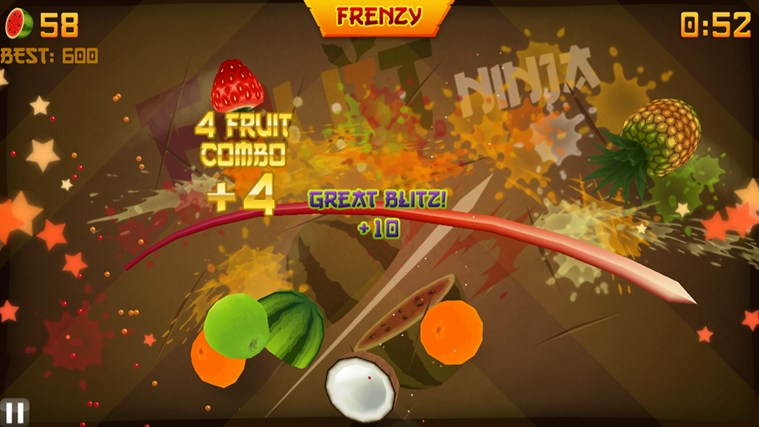
\includegraphics[width=0.49\linewidth]{images/ch10/4} \hfill
	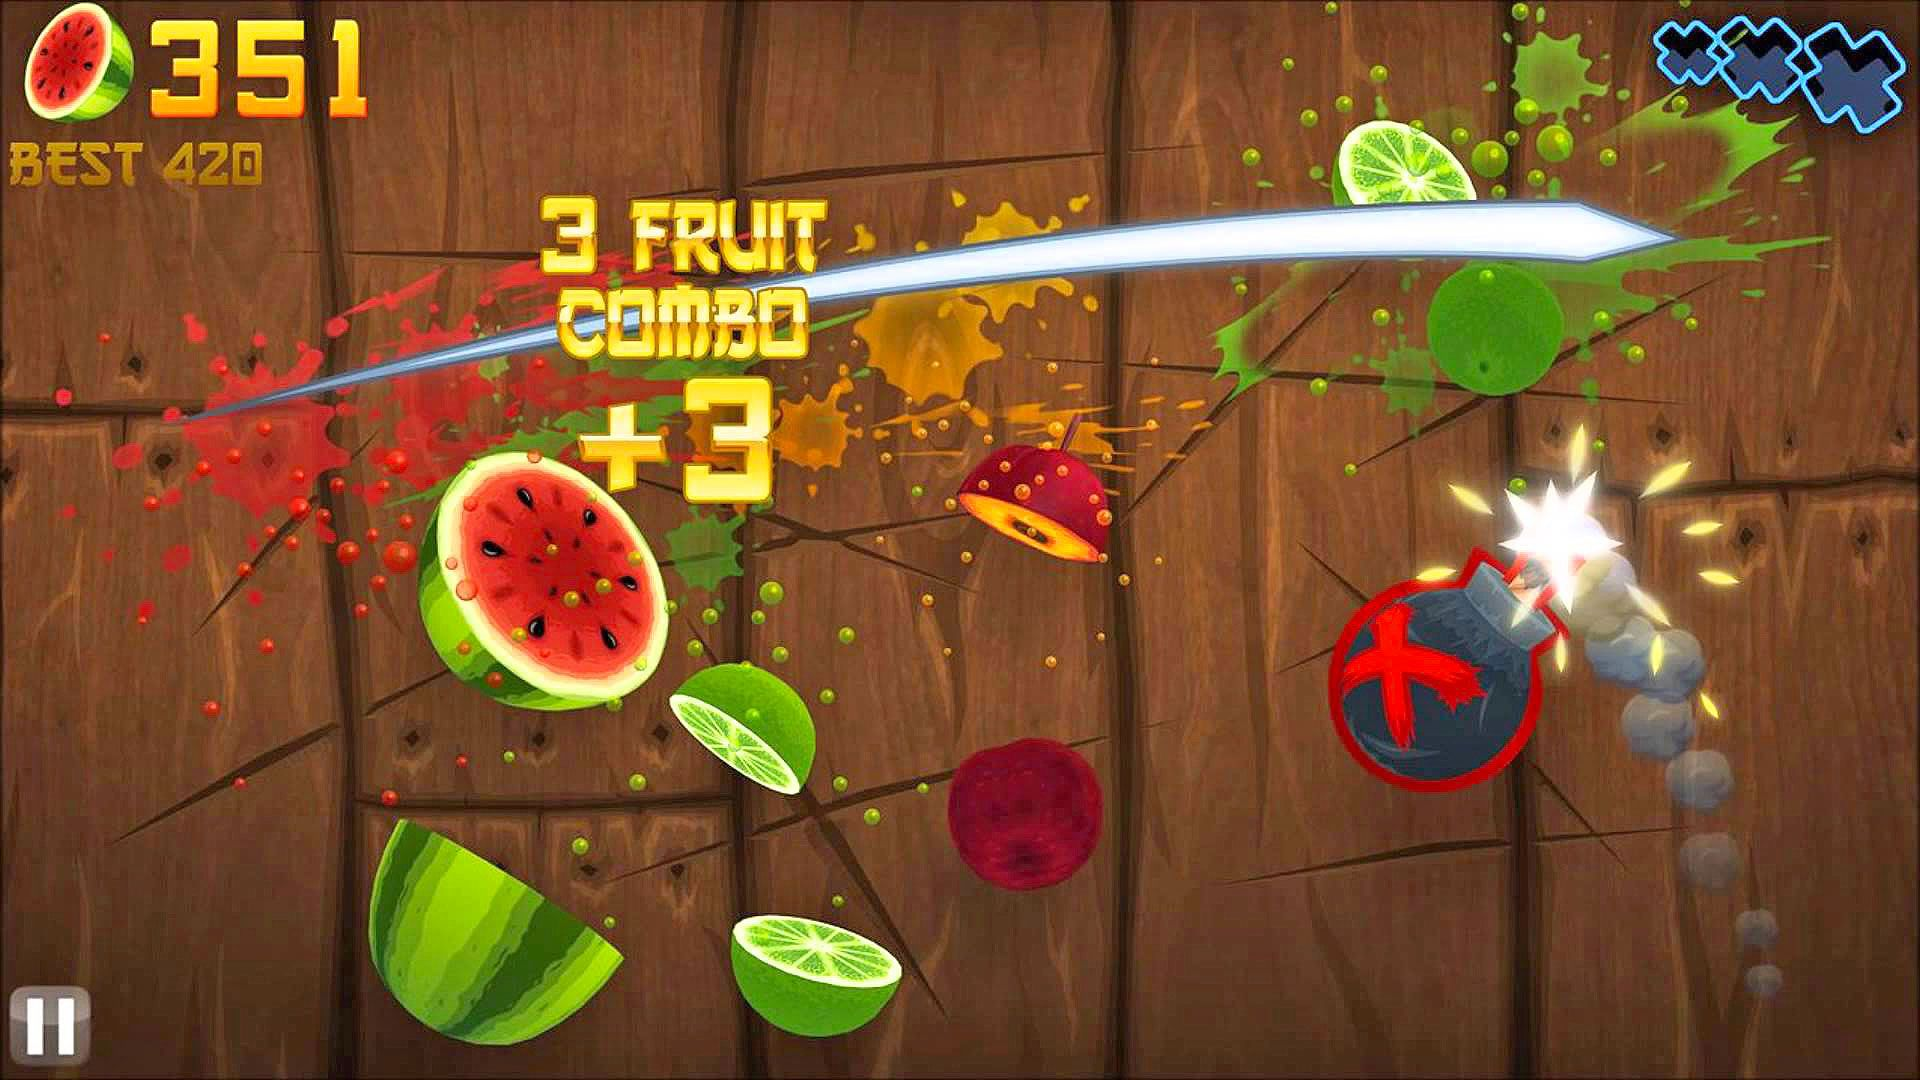
\includegraphics[width=0.49\linewidth]{images/ch10/1}
	\\[0.15cm]
	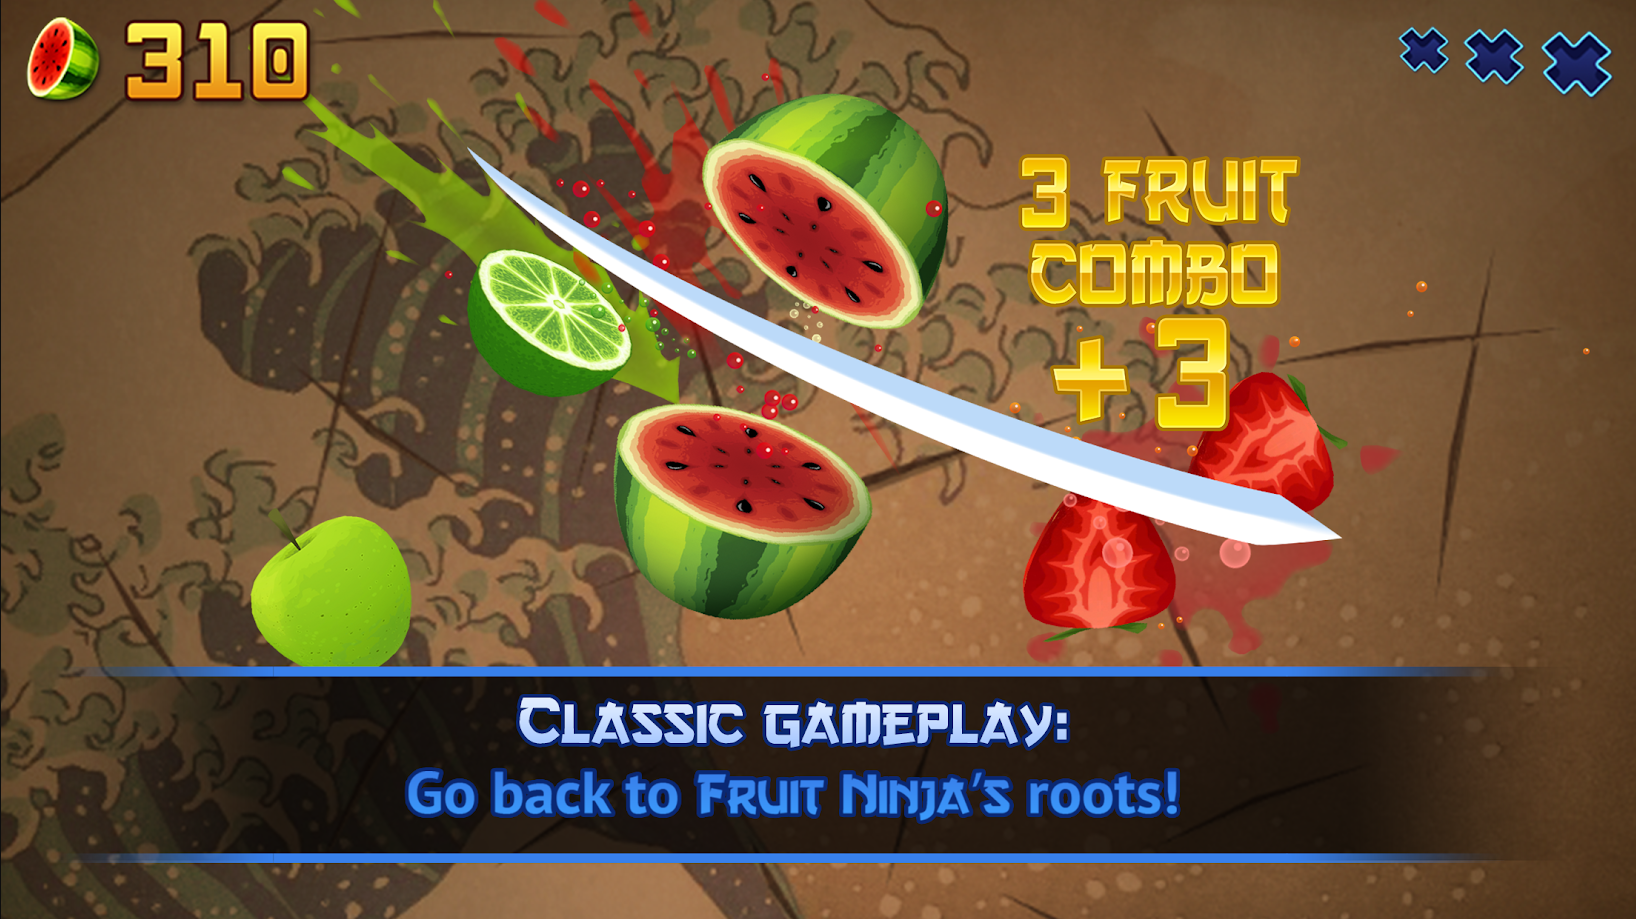
\includegraphics[width=0.49\linewidth]{images/ch10/2} \hfill
	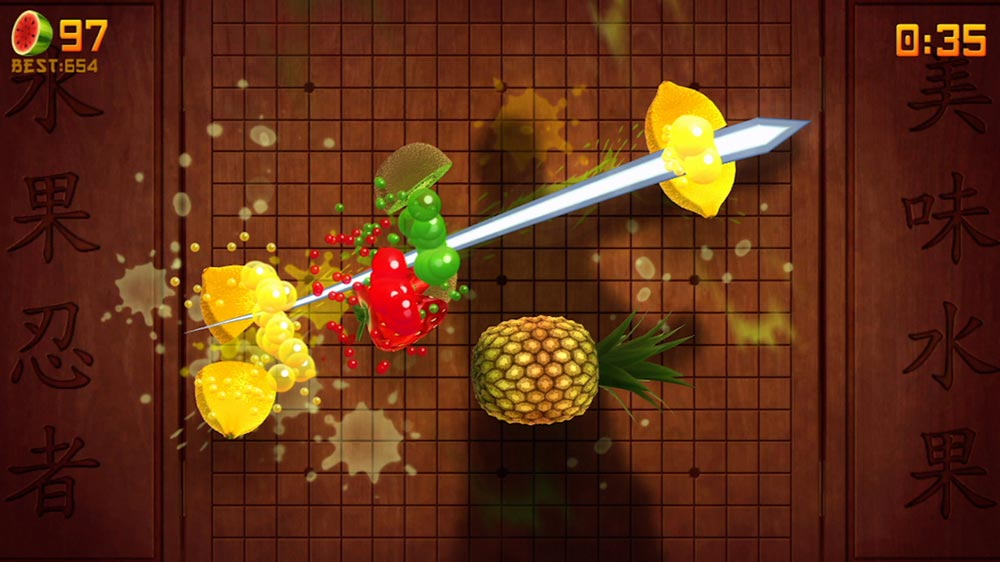
\includegraphics[width=0.49\linewidth]{images/ch10/3}	
	
	\caption{Esempio di alcune versioni e modalità di gioco di Fruit Ninja. Da sinistra verso destra abbiamo (1) Screen della prima versione originale, (2) Versione HD, (3) Ultima versione con un ritorno al passato, (4) Versione VR. }
\end{figure}

Fruit Ninja mette a disposizione diverse modalità di gioco che si basano tutte sul gameplay appena descritto:
\begin{itemize}
\item \textbf{Classica}: Il giocatore ha a disposizione tempo illimitato e 3 vite, insieme ai frutti possono essere lanciate anche delle bombe esplosive da evitare. Ogni frutto mancato causa la perdita di una vita, se si colpisce una bomba oppure si perdono tutte le vite il gioco terminerà. Ogni cento punti si guadagna una vita. Non ci sono limiti alla durata della partita o del punteggio se non la bravura del giocatore.
\item \textbf{Arcade}: Dura 60 secondi, l'obiettivo è battere il record. Le differenze dalla modalità classica sono: il tempo è limitato, non vi sono vite\sidenote{la frutta mancata non causa effetti negativi.} e per ogni bomba colpita il tempo rimasto viene diminuito di 10 secondi. Sono inoltre presenti banane speciali con effetti speciali che conferiscono brevi bonus quando tagliate.
\item \textbf{Zen}: Nella modalità Zen, la durata della partita è di 1:30 minuti l'obiettivo è battere il record, non saranno presenti bombe e vite e si dovrà quindi unicamente cercare di affettare più frutta possibile puntando sulle combo senza l'ausilio di bonus. 
\end{itemize}
Per lo sviluppo del progetto si è scelta come base la \textbf{modalità Zen}.





\section{Fruit Ninja GL}
\begin{marginfigure}
	
\includegraphics[width=\linewidth]{images/ch10/6}
	\caption{Logo della software di fantasia che ha sviluppato il fnGL.}
\end{marginfigure}
In questa relazione verrà descritto \textbf{Fruit Ninja GL} (da ora in poi abbreviato con \textbf{fnGL}) clone sviluppato in OpenGL dalla \textbf{\textit{Space Mambo Studios}} un'immaginaria software house. L'idea di base è quella di replicare la modalità Zen del gioco integrandola però di alcune caratteristiche mancanti\sidenote[*+2][]{Nel gioco originale, mancano totalmente Luci e Collisioni tra i frutti i quali semplicemente si sovrappongono.} ma necessarie ai requisiti del progetto senza però snaturare o alterare il gameplay originale.

\begin{figure}[!htp]
	\centering
	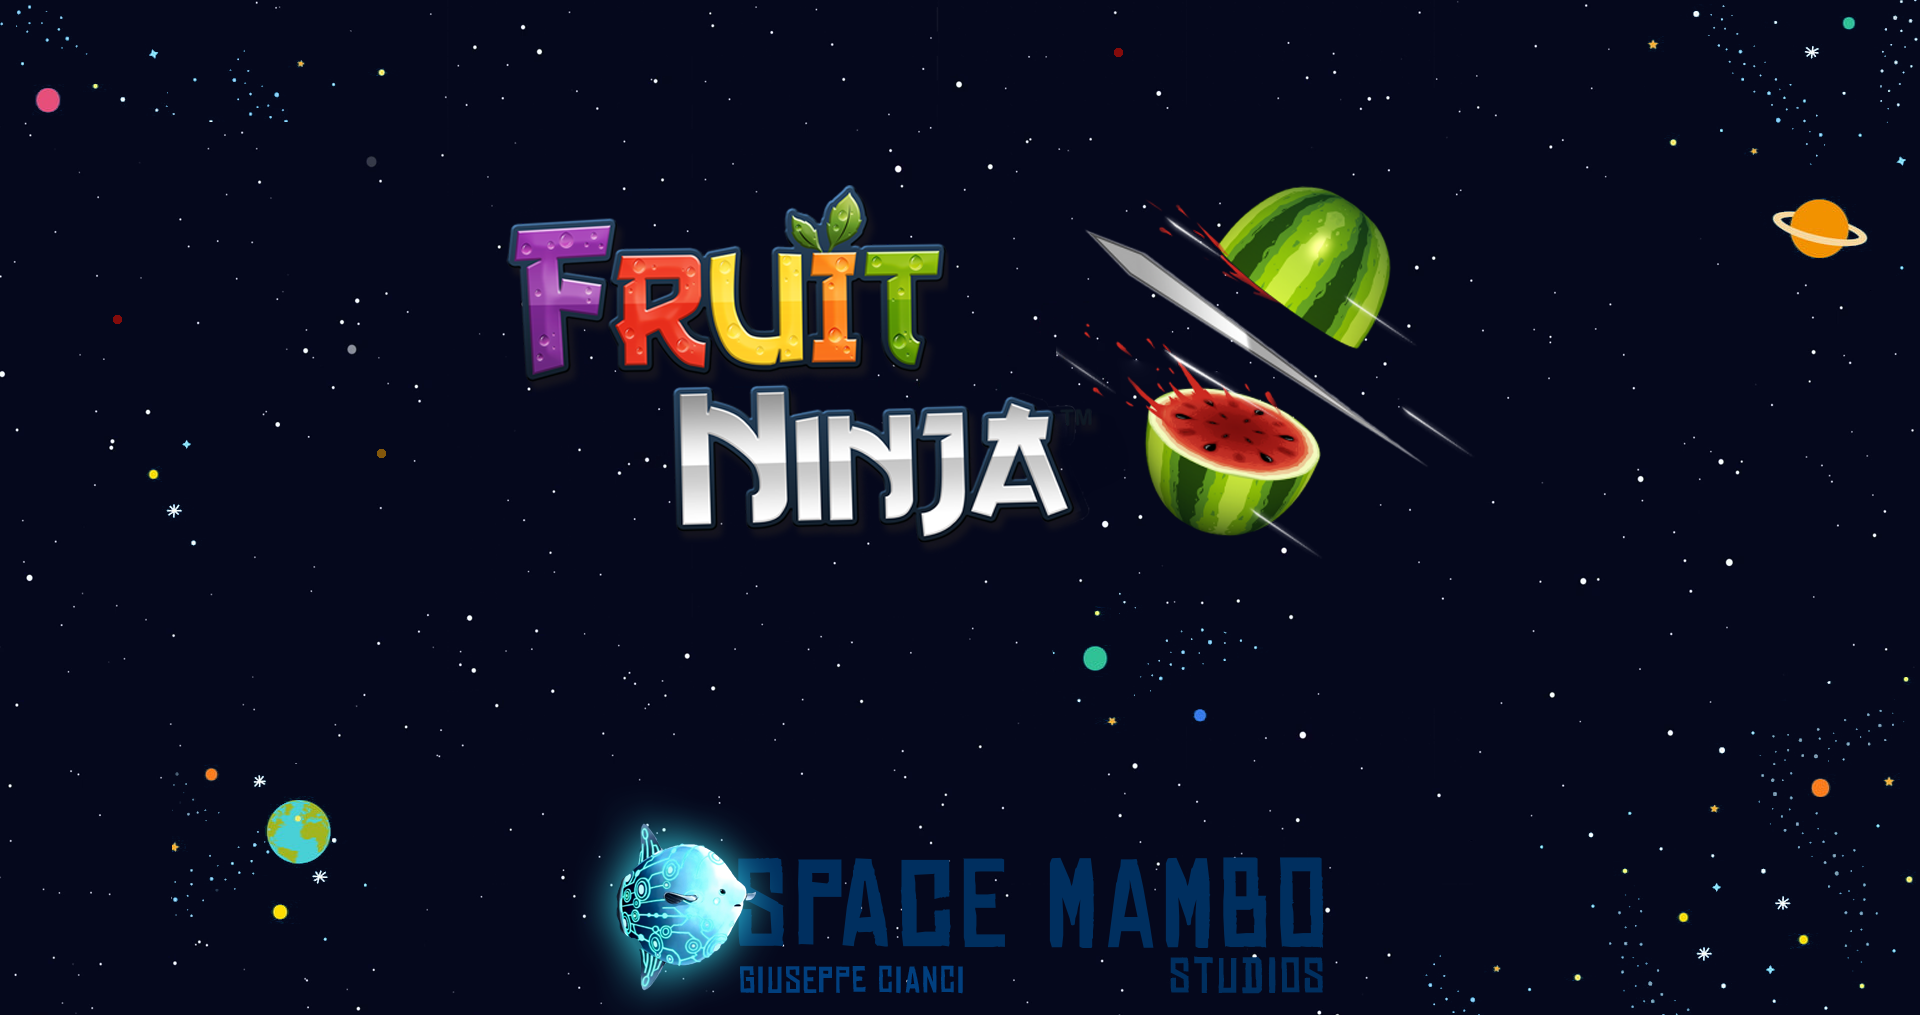
\includegraphics[width=0.49\linewidth]{images/ch10/a2} \hfill
	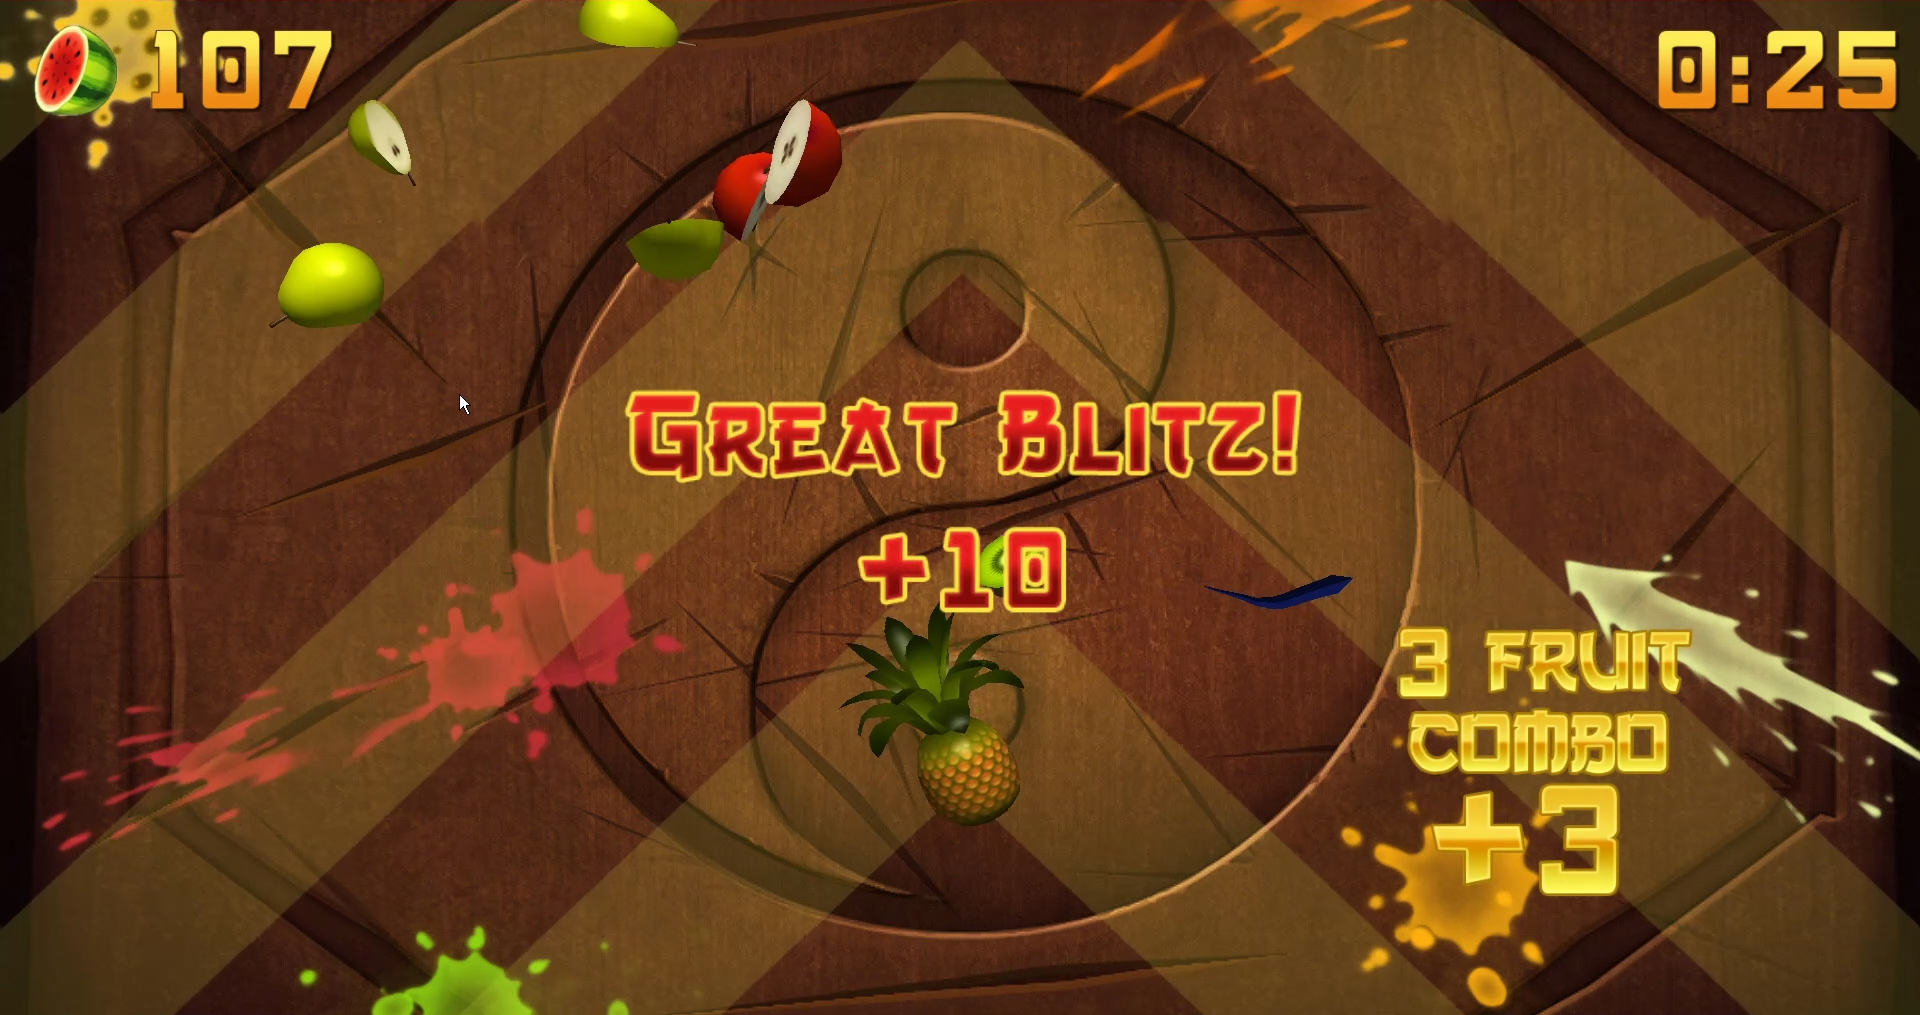
\includegraphics[width=0.49\linewidth]{images/ch10/a1}
	\\[0.15cm]
	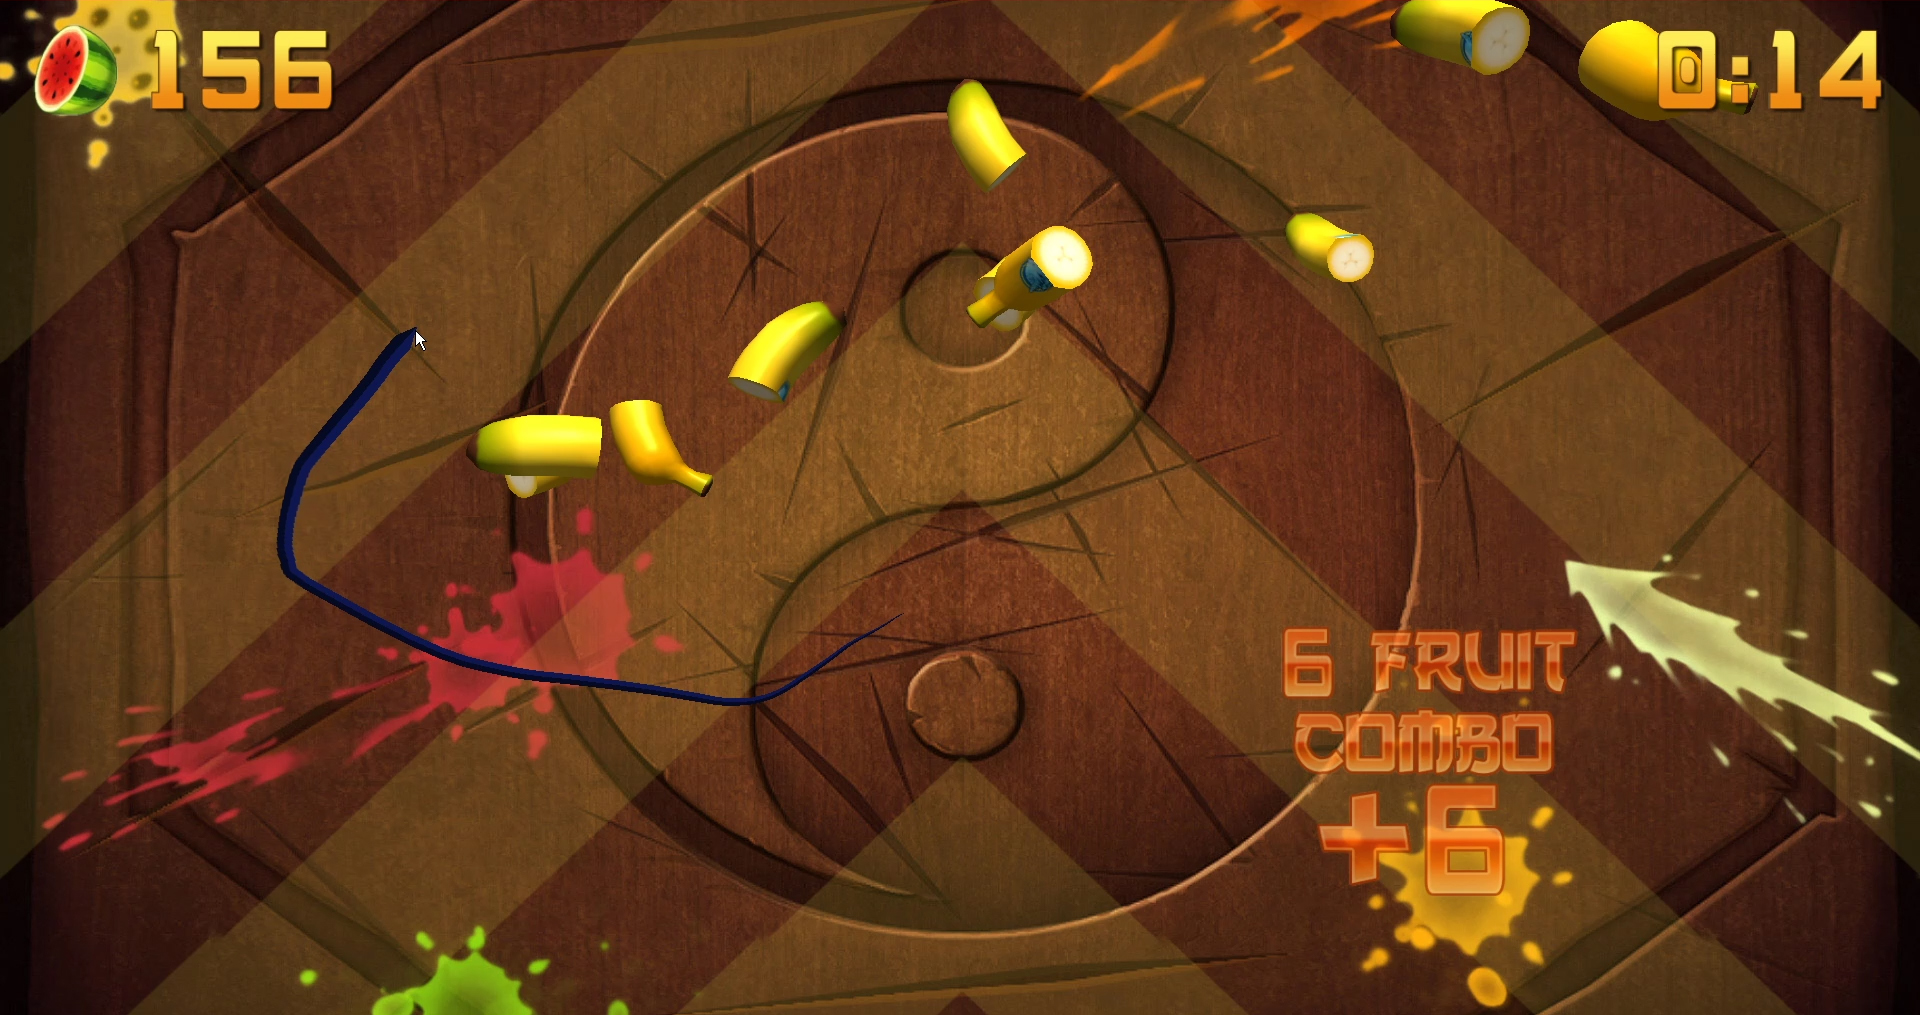
\includegraphics[width=0.49\linewidth]{images/ch10/a3} \hfill
	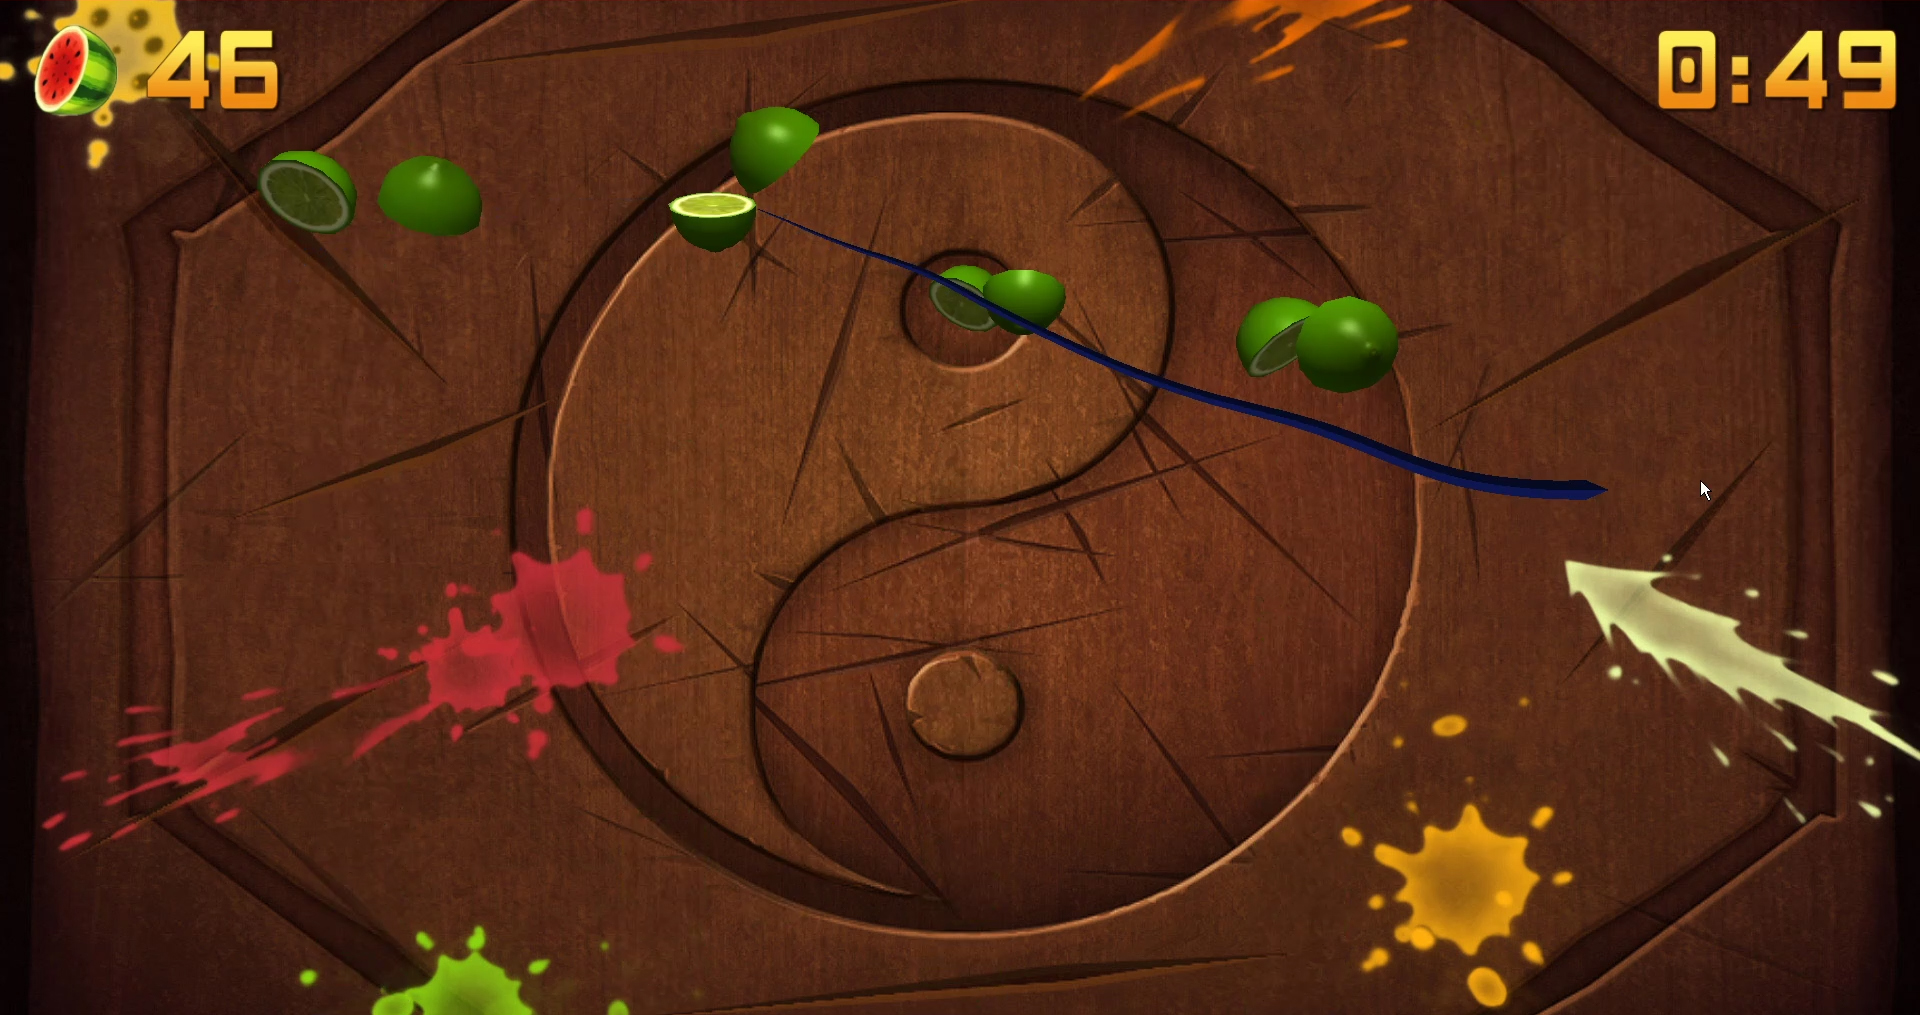
\includegraphics[width=0.49\linewidth]{images/ch10/a4}	
	
	\caption{Alcuni screen di gioco di Fruit Ninja GL.}
\end{figure}

Il giocatore avrà a disposizione 1:30 minuti per affettare quanti più punti possibili effettuando \textit{combo} e \textit{blitz} per massimizzare il punteggio finale. A completare il tutto sono presenti le musiche e gli effetti originali del gioco cercando di replicare nel dettaglio anche la grafica.

\subsection{Librerie e Software Utilizzati}
Fruit Ninja GL è stato sviluppato utilizzando C++20 in ambiente Visual Studio ed è basato sull'ultima versione disponibile di OpenGL la 4.6; Oltre a ciò sono state impiegate diverse librerie o moduli per semplificare lo sviluppo del gioco:
\begin{itemize}
\item \texttt{GLFW} \cite{GLFW}: Libreria open-source, multi-piattaforma per OpenGL. Fornisce una semplice API per la creazione di finestre, contexts e la gestione di diverse tipologie input ed eventi.

\item \texttt{GLEW} \cite{GLEW}: Libreria multi-piattaforma open-source per il loading delle funzioni OpenGL. Fornisce un meccanismo moderno ed efficiente per determinare, a run-time, quale estensione di OpenGL è supportata dalla piattaforma target. 

\item \texttt{GLM} \cite{GLM}: Libreria matematica basata sulle specifiche\sidenote{Le funzionalità non sono però limitate al GLSL ma si estendono anche alle trasformazioni matriciali, quaternioni, data packing, random numbers, noise, etc...} del OpenGL Shading Language (GLSL). 

\item \texttt{ASSIMP} \cite{ASSIMP}: Libreria open-source che fornisce una API semplice ed unificata per la gestione di vari formati di modelli 3D, in particolare consentendone il caricamento, lattura oltre che l'esportazione. 

\item \texttt{stb\_image} \cite{STB}: Libreria open-source che consente il loading/decoding da file o memoria di immagini nei formati più comuni.

\item \texttt{irrKlang} \cite{IRRKLANG}: Libreria ad alto livello che consente il caricamento e l'esecuzione di numerosissimi formati audio.

\item \texttt{\{fmt\}} \cite{FMT}: Libreria open-source per il format delle stringhe. 

\item \texttt{ImGUI} \cite{IMGUI}: Libreria per il disegno di GUI interattive \sidenote{Utilizzata nelle fasi iniziali di sviluppo più per un rapido debug e prototipazione. Rimossa nelle fasi finali del progetto.}. 
\end{itemize} 

Inoltre è stato utilizzato \textbf{Visual Studio 2019} per lo sviluppo, \textbf{Adobe Photoshop} per la creazione di sprite e l'editing di texture ed in fine \textbf{Doxygen} + \textbf{m.css}\footnote{A modern, mobile friendly drop-in replacement for the stock Doxygen HTML output. \url{https://mcss.mosra.cz/mcss/documentation/doxygen/}} per la produzione della documentazione.


\subsection{Documentazione}
Tutto il codice è ben documentato e correlato di una documentazione prodotta dai commenti che descrive i vari moduli, classi e funzioni implementati.

\begin{figure}[!htp]
	\centering
	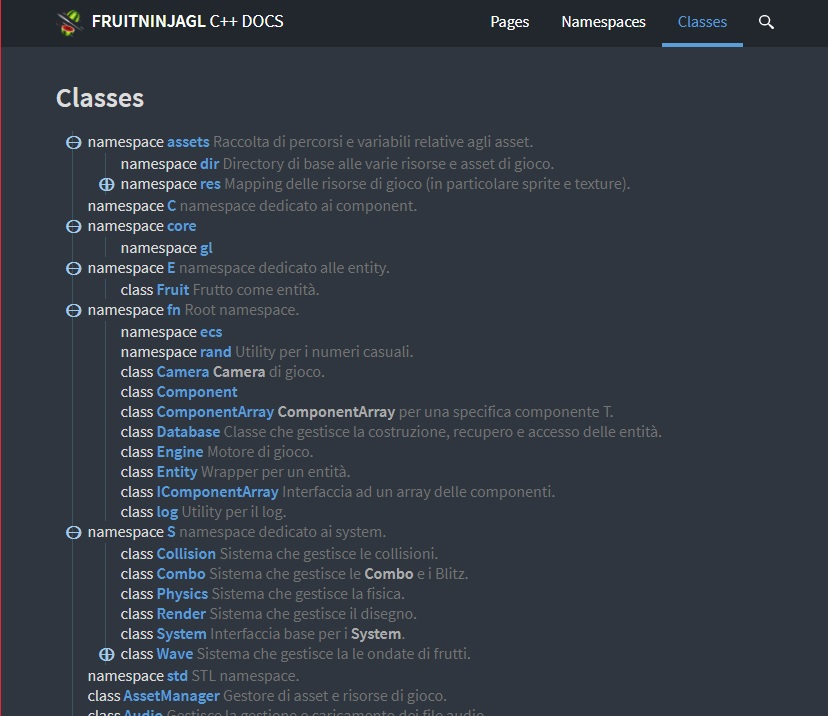
\includegraphics[width=0.9\linewidth]{images/ch10/5}
	\caption{Esempio della documentazione prodotta con Doxygen + m.css. Nella figura è mostrata la lista della classi. }
\end{figure}




\subsection{Avvio dell'applicazione}
Per poter avviare l'applicazione è necessario effettuare una sorta di processo di installazione\sidenote{L'ultima versione dell'eseguibile è già stata spostata ed è attualmente presente.}.

Una volta compilata l'applicazione l'eseguibile generato va spostato all'{}interno della cartella \texttt{./FruitNinjaGL/FruitNinjaGL/} ovvero quella dove sono presenti i file di progetto VisualStudio; Tale operazione è fondamentale per accedere ai file \texttt{.dll} per il linking delle librerie e alla cartella \texttt{./res} contenente tutti gli asset e risorse di gioco i cui percorsi sono relativi alla workspace del progetto.





















































%

















\setchapterpreamble[u]{\margintoc}
\chapter{Fruit Ninja GL}

\begin{chap-intro}
	In questo capitolo si descriverà nel dettaglio il progetto d'esame, effettuando prima una breve overview sulle principali caratteristiche e scelte implementative ed architetturali per poi successivamente passare ai vari dettagli implementativi.
\end{chap-intro}

\section{Overview}
Fruit Ninja GL è basato in OpenGL 4.6 Core Profile utilizzando la libreria GLFW 3.3.2 per la crazione del contesto, finestra e gestione di input ed eventi. L'applicazione è stata sviluppata in C++20 in ambiente Visual Studio\sidenote{Il codice è compilabile in ambiente linux utilizzando un altro compilatore.} 2019.

\subsubsection{Simile all'originale}
\begin{marginfigure}
	\centering
	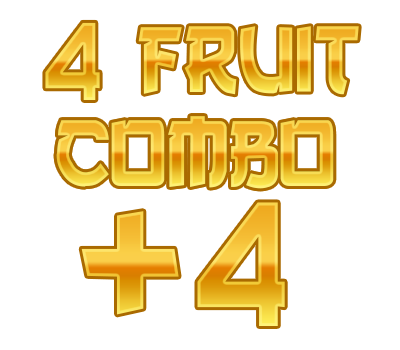
\includegraphics[width=0.7\linewidth]{images/ch20/0}
	\caption{Esempio di sprite realizzato imitando lo stile di Fruit Ninja.}
	\label{fig:combo4}
\end{marginfigure}
Durante lo sviluppo si è cercati di rimanere il più possibile fedeli al gioco nella sua versione originale rilasciata nel 2010. Musiche, suoni, font e sfondi sono liberamente disponibili in rete mentre gli sprite ed elementi della GUI sono stati riprodotti utilizzando photoshop\footnote{Tutti i file \texttt{.psd} creati ed utilizzati sono inclusi assieme agli asset.}.

I modelli 3D dei frutti sia nella loro versione \enquote{intera} che \enquote{affettata} sono presi da uno dei tanti Fruit pack disponibili in rete.


\subsubsection{Entity Component System}
Lo sviluppo delle logiche di gioco è stato basato sull'Entity Component System, un pattern architetturale molto comune nel game development\sidenote{Utilizzabile in molti motori grafici come Unity, Unreal Engine o il Cryengine.}


\subsubsection{Astrazione delle primitive}
Tutte le principali primitive grafiche (di OpenGL e non) come \textit{texture}, \textit{mesh}, \textit{model}, \textit{shader} o \textit{audio} sono state astratte in specifiche classi per rendere più semplice, immediato e conveniente il loro utilizzo.


\subsubsection{VAOs, VBOs, Vertex e Shaders}
\marginnote{
Si è scelto questo approccio invece che la semplice \textit{direct API mode} (\texttt{glBegin()}, \texttt{glEnd()}, ...) perché quest'ultima è deprecata (e dunque nemmeno disponibile nel  Core Profile), molto più lenta oltre che poco \enquote{compatibile} con il loading di asset e modelli 3D complessi.
}
Il rendering dei vari oggetti è effettuato ricorrendo ai vari buffer (Vertex Array Object, Vertex Buffer Array, Index Buffer Array) e Shaders (Vertex e Fragment) di OpenGL. Sono stati implementati diversi shader a seconda dell'elemento grafico o di come lo si vuole disegnare nel framebuffer.

Dopo una iniziale difficoltà l'utilizzo dei buffer unito con gli shader rende lo sviluppo più semplice e flessibile.


\subsubsection{Engine a Stati}
L'engine di gioco è basato sul Game State 'Stack' un altro pattern architetturale molto diffuso per la gestione dei vari possibili stati di gioco (Loading, playng, pause, game over, ...).


\section{Descrizione Architetturale}
Architetturalmente Fruit Ninja GL è strutturato in cinque \textit{macro-moduli} ognuno dei quali si occupa di gestire una parte dell'applicazione. 
\begin{itemize}
	\item \texttt{core/} classi finalizzate alla gestione dei dettagli a basso livello di OpenGL e non.
	\item \texttt{ecs/} implementazione dell'ECS con componenti, sistemi e relative classi di gestione delle entità.
	\item \texttt{engine/} implementazione del motore di gioco a stati.
	\item \texttt{logic/} dettagli relativi al gameplay e agli elementi di gioco.
	\item \texttt{utl/} classi e funzioni di utility o debug.
\end{itemize}

\subsection{Modulo \texttt{core/}}
Il modulo \texttt{core} contiene tutta una serie di classi e funzioni con il principale scopo di astrarre il più possibile le funzionalità a basso livello messe a disposizione da OpenGL e da altre librerie. L'idea è quella di creare una serie di API semplici su cui si baserà l'intera applicazione.

\begin{figure}[!hpt]
	\centering
	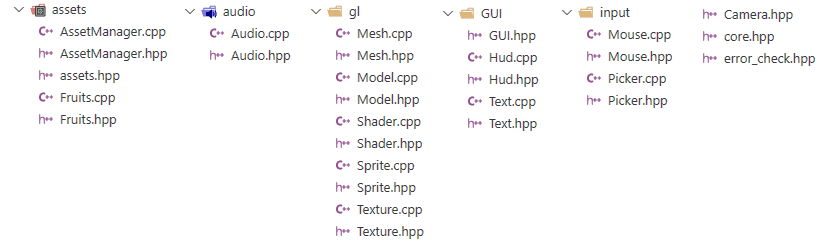
\includegraphics[width=\linewidth]{images/ch20/1}
	\caption{Sotto-moduli e relativi file \texttt{.hpp} e \texttt{.cpp} che fanno parte di \texttt{core}.}
	\label{fig:module-core}
\end{figure}

Come è possibile vedere in figura \rref{fig:module-core} \texttt{core} è strutturato in sotto-moduli ognuno con funzionalità specifiche; nella root principale invece è presente:
\begin{itemize}
\item \texttt{Camera.hpp} una semplice classe che gestisce la camera posizionandola nello spazio e costruendo di conseguenza la \textit{projection matrix} (prospettica) e la \textit{view matrix}.
\item \texttt{error\_check.hpp} contiene macro e callback per il debug ed il checking di errori di OpenGL.
\end{itemize}

\subsubsection{Sotto-modulo \texttt{asset}}
\begin{marginfigure}%[!hpt]
	\centering
	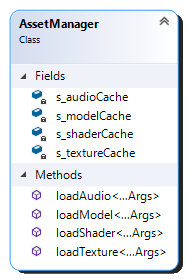
\includegraphics[width=0.8\linewidth]{images/ch20/2}
	\caption{Diagramma UML della classe AssetManager}
\end{marginfigure}
Dedicato alla gestione di asset e risorse grafiche/multimediali di gioco. Oltre alla semplice definizione di cartelle e percorsi (\texttt{asset.hpp}) o alla strutturazione di asset composti (\texttt{fruit.hpp}) nel modulo si implementa anche un \textit{gestore degli asset} (\texttt{AssetManager.hpp}) che utilizzando il patter flyweight consente di caricare e riutilizzare in maniera veloce e dinamica le varie risorse di gioco fornendo lo stesso puntatore ogni qual volta quella risorsa è richiesta.

Tutti gli asset inoltre hanno costruttori di copia e assegnazione disabilitati per evitare duplicazione di risorse.

\begin{cpp}[caption={Esempio di metodo utilizzata dal manager per il caricamento dei Modelli.}, captionpos=t]
template<typename ...Args>
inline constexpr ModelSP AssetManager::loadModel(const fs::path& filepath, Args && ...args)
{
	// Verifico che il modello non sia in cache
	auto f = filepath.string();
	if (AssetManager::s_modelCache.find(f) != AssetManager::s_modelCache.end())
	return AssetManager::s_modelCache[f];
	
	auto model = std::make_shared<Model>(filepath, std::forward<Args>(args)...);
	AssetManager::s_modelCache[f] = model;
	return model;
}
\end{cpp}


\subsubsection{Sotto-modulo \texttt{audio}}
Dedicato alla gestione delle funzionalità audio sia 2D che 3D dell'{}applicazione ricorrendo alla libreria irrKlang \cite{IRRKLANG}. La classe \texttt{Audio} è considerata come un asset di gioco, si occupa del caricamento nonché dell'esecuzione dei file audio e fornisce metodi statici per la gestione generale\sidenote{Ad esempio per interrompere tutti i suoni in esecuzione o semplicemente abbassare il volume.}.


\subsubsection{Sotto-modulo \texttt{gl}}
Dedicato all'astrazione delle principali primitive di OpenGL in modo da consentine un uso facile e componibile. 
\begin{itemize}
\item \texttt{Texture}: gestisce il loading, creazione e binding delle texture. Il caricamento del file in sè avviene tramite la libreria \texttt{stb\_image} \cite{STB} mentre la creazione e binding openGL è effettuato al caricamento supporta anche eventuali parametri. La classe è anche un asset.
\begin{cpp}
Texture::Parameteri parm = {
	{ GL_TEXTURE_WRAP_S, GL_MIRRORED_REPEAT },
	{ GL_TEXTURE_WRAP_T, GL_MIRRORED_REPEAT },
	{ GL_TEXTURE_MIN_FILTER, GL_NEAREST },
	{ GL_TEXTURE_MAG_FILTER, GL_NEAREST },
};
this->m_texture = AssetManager::loadTexture(filepath, parm);
\end{cpp}

\item \texttt{Mesh}: gestisce una singola Mesh + texture. I dati sono rappresentati utilizzando le strutture e buffer di OpenGL. La classe definisce anche la struttura e layout dei vertici\sidenote{Tale struttura è quella che poi è utilizzata in ogni elemento 3D.}.

\item \texttt{Model}: gestisce un Modello, ovvero una composizione di più mesh. Il caricamento dei modelli dal disco avviene utilizzando la libreria ASSIMP \cite{ASSIMP}.

\item \texttt{Shader}: gestisce gli shader\sidenote{Uno \texttt{Shader} è composto da un vertex shader e da un fragment shader.} di OpenGL, la classe ne consente il caricamento del sorgente \texttt{.glsl}, la compilazione, il linking ed in fine l'attivazione o disattivazione.
\end{itemize}

\subsubsection{Sotto-modulo \texttt{input}}
Dedicato alla gestione degli input utente. 
\begin{itemize}
	\item \texttt{Mouse}, singleton tramite il quale ogni altro componente può sapere quale pulsante è stato premuto e le ultime posizioni assunte dal mouse durante il trascinamento nella finestra creata da GLFW.
	\item \texttt{Picker}, classe speciale che consente di effettuare il picking delle entità disegnate sul framebuffer.
\end{itemize}


\subsection{Modulo \texttt{ecs/}}
Il modulo \texttt{ecs} implementa il pattern architetturale Entity Component System.

\begin{figure}[!hpt]
	\centering
	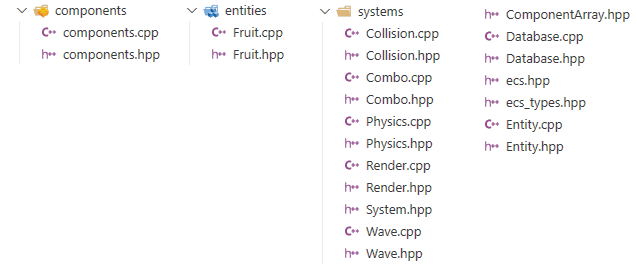
\includegraphics[width=0.95\linewidth]{images/ch20/3}
	\caption{Sotto-moduli e relativi file \texttt{.hpp} e \texttt{.cpp} che fanno parte di \texttt{ecs}.}
	\label{fig:module-ecs}
\end{figure}

Il funzionamento, le classi e eventuali dettagli implementativi verranno descritti nella sezione \rref{sec::ecs}.


\subsection{Modulo \texttt{engine/}}
Il modulo \texttt{engine} implementa il pattern architetturale Game state ``stack" per la gestione degli stati di gioco ed il game loop.

\begin{figure}[!hpt]
	\centering
	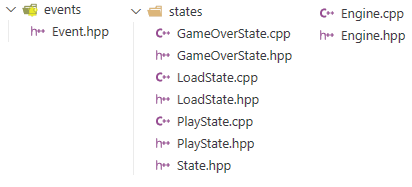
\includegraphics[width=0.8\linewidth]{images/ch20/4}
	\caption{Sotto-moduli e relativi file \texttt{.hpp} e \texttt{.cpp} che fanno parte di \texttt{engine}.}
	\label{fig:module-engine}
\end{figure}

La classe principale per il funzionamento di tutta l'applicazione è \texttt{Engine} ovvero il motore di gioco. Engine è un singleton che ha il compito di inizializzare l'intera applicazione (moduli, sotto-moduli, contesti e librerie) per poi avviare il game loop sullo stato correntemente in cima allo stack degli stati.

\begin{cpp}[caption={Funzione che esegue un singolo loop di gioco. Una volta determinato il 
 tempo trascorso dall'ultima iterazione in ordine: si effettua il polling degli eventi (glfw), si gestisce l'input, si aggiorna lo stato interno, si effettua il rendering ed in fine si gestiscono gli eventi di gioco.
}, captionpos=t]
void Engine::loop() {
	auto now = core::seconds(glfwGetTime());  
	this->delta_t = now - last_t;
	last_t = now;                  // Determino il tempo trascorso
	Mouse::update(this->delta_t);  // Aggiorno Mouse
	
	if (m_states.empty()) return;
	auto& state = *m_states.top(); // Prendo lo stato corrente
	
	glfwPollEvents();              // Handle inputs
	state.handleInputs();
	state.update(this->delta_t);   // Update
	state.render();                // Render
	state.handleEvents();          // Handle Events
}
\end{cpp}

La classe non conosce nulla riguardo il gioco in se ma si limita semplicemente ad aggiornare lo stato correntemente attivo che conterrà tutte le logiche di funzionamento.

\subsection{Modulo \texttt{utl/}}
Il modulo \texttt{utl} contiene delle semplici funzioni di utility per il print, logging (utilizzando la libreria \texttt{\{fmt\}}) e la generazione di numeri e/o vettori casuali (utilizzando la libreria \texttt{glm}).

\section{Entity Component System}
\label{sec::ecs}
Entity–component–system (ECS) è un pattern architetturale estremamente diffuso nel game development, \marginnote{L'idea di utilizzare questo pattern per strutturare fnGL è stato più uno sfizio personale che una vera necessità.} incorporato nativamente in molti dei game engine più comuni vantando elevate prestazioni, grande flessibilità e semplicità di progettazione. 

Come dice il nome, tre sono i concetti fondamentali:

\begin{itemize}
	\item \textbf{Entity}: Sono elementi ``general porpouse" del gioco, possono essere qualsiasi cosa\sidenote{Es. nemici, sprite, particelle, effetti, animazioni, ...} ogni entity è identificata da un id univoco.

	\item \textbf{Components}: Sono i raw data rappresentanti un singolo aspetto/caratteristica di un'entità \sidenote{Es. posizione, velocità, mesh, AABB, AI, tags, stato, ...}. Ad una singola entità è possibile associare più componenti. Anch'essi sono identificati univocamente con un id.
	
	\item \textbf{System}: Contengono la logica di un singolo aspetto atomico del gameplay\sidenote{Es. Gravità, Collisioni, Spawn, Movimento, Rendering, ...}, e processano tutte le entità che possiedono le componenti richieste dal sistema. La ricerca delle entità compatibili è detta \textbf{\textit{query}}.
\end{itemize}

\marginnote{Si evitano così anche alcuni problemi tipici dell'OOP come le gerarchie profonde, l'eredità multipla, la flessibilità, e la generalizzabilità.}
L'ECS segue il \textit{composition over inheritance principle} ovvero si preferisce definire le caratteristiche degli oggetti (entity) attraverso la composizione (components) e non mediante l'ereditarietà. Ciò conferisce un'enorme flessibilità nello sviluppo dal momento che il comportamento delle entità (systems) può facilmente essere cambiato a runtime semplicemente rimuovendo o modificando i suoi componenti.

Un'ulteriore punto chiave dell'ECS è il \textbf{data-oriented design}, ovvero un approccio di strutturazione del codice orientato ai dati (piuttosto che agli oggetti) al fine di ottimizzare quanto più possibile l'utilizzo della cache della CPU focalizzandosi sul layout dei dati, scomposizione degli oggetti, località dei dati etc...

\subsection{Database}
Per completare il funzionamento del pattern è in realtà necessario un ulteriore elemento il \textbf{Database}\sidenote{Anche chiamato world, universe o enetity manager.}. Come è facile intuire dal nome, il database ha il compito di creare le entità fornendo loro identificativi univoci, tenere traccia dei componenti assegnati ad esse ed in fine eseguire query e ricerche per i sistemi. Il tutto cercando di mantenere un approccio data-oriented.

\begin{emptyBox}
L'implementazione dell'ECS di Fruit Ninja GL è fortemente ispirato (per API e filosofia) ai framework più famosi in particolare ad \texttt{\textit{entt}} utilizzato per minecraft, \texttt{\textit{ecsX}} e \texttt{\textit{flecs}}. Tutte queste implementazioni fanno forte uso di template, variatics, constexpr e altre funzionalità avanzate del C++.
\end{emptyBox}

Nelle seguenti sezione si procederà a descrivere i vari elementi dell'ECS implementati nel framework di fnGL. Infine nella sezione \rref{ssec:example-ecs} si mostreranno alcuni esempi di utilizzo.

\subsection{Entità}
In fnGL una entity è un \cppinline{fn::Eid} ovvero un identificativo univoco che altri non è che un \cppinline{unsigned int}. Tutte le entità devono essere generate da un database\sidenote{Più database sono possibili ma in quel caso è necessario non mischiare le entità create fra le varie istanze.} e non possono essere create in altri modi.

\begin{cpp}
 Database database();
 fn::Eid e1 = database.create<fn::Eid>();        // (1)
 E::Entity e2 = database.create<E::Entity>();    // (2)
 E::Entity e3 = database.create();               // (3)
\end{cpp}

La creazione avviene semplicemente utilizzando il metodo \cppinline{create<>} tramite la quale come un template è possibile specificare come deve essere restituita l'entità:
\begin{enumerate}
\item Crea l'entità e restituisce semplicemente il suo identificativo.
\item Crea l'entità ma restituisce un oggetto \cppinline{E::Entity} che banalmente contiene internamente il \cppinline{fn::Eid}.
\item Uguale al metodo (2), \cppinline{E::Entity} è la tipologia di default.
\end{enumerate}


\subsubsection{\texttt{E::Entity}}
Dal momento che l'Eid è un semplice intero, senza il suo database di appartenenza risulta ovviamente poco utile. Per questo motivo, per comodità, è stata creata la classe \cppinline{E::Entity} ovvero un semplice wrapper che contiene sia l'identificativo che un puntatore al database. 

Tramite un \cppinline{E::Entity} sono richiamabili tutti i metodi del database che contiene senza ovviamente la necessità di dover specificare anche l'Eid.

\subsubsection{\texttt{E::Fruit}}
La classe \cppinline{E::Fruit} deriva da \texttt{E::Entity} e ne condivide principi e funzionamento di base. L'unica differenza è che mette a disposizione una serie di metodi ed attributi statici di utility per la manipolazione di questo tipo di entità sempre per mezzo del database.

Si tratta quindi di una semplice classe che racchiude alcune logiche del gioco.

\begin{figure}[!htp]
	\centering
	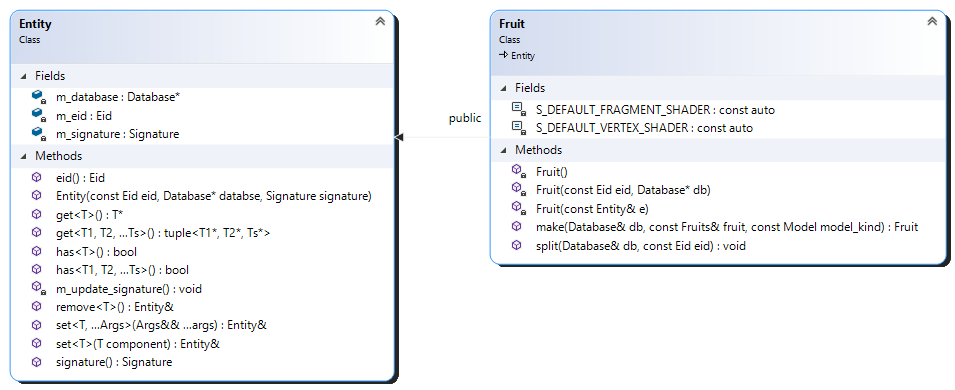
\includegraphics[width=0.95\linewidth]{images/ch20/5}
	\caption{Diagramma UML delle classi Entity e Fruit}
	\label{fig:5}
\end{figure}



\subsection{Componenti}
\marginnote{Tutte le componenti si trovano sotto il \cppinline{namespace C}.}
In fnGL un component è una qualsiasi struct/class che estende \cppinline{struct} \cppinline{Component<T>} ed è inizializzabile tramite initialization list. Le componenti, per garantire la località dei dati dovrebbero essere dei POCO\footnote{Cioè dei 
Plain Old C++ object ovvero delle semplici classi o struct che memorizzando lvalue di tipi primitivi o aggregati di primitivi.} il cui contenuto è il dato stesso e non un puntatore o un reference. 

\begin{figure}[!htp]
	\centering
	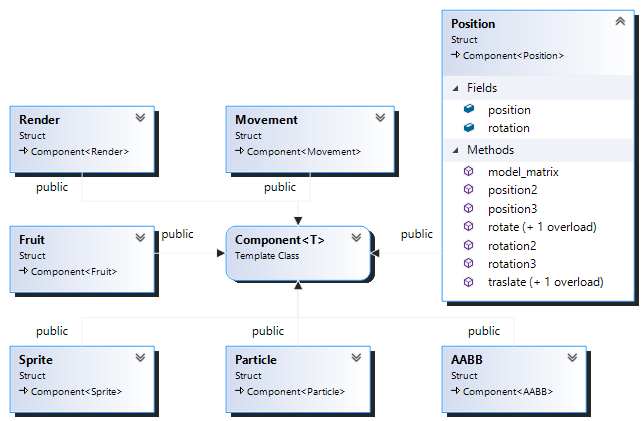
\includegraphics[width=0.95\linewidth]{images/ch20/6}
	\caption{Diagramma UML di tutte le componenti implementate in fnGL. Come è possibile vedere dal dettaglio di \texttt{C::Position} oltre ai dati in realtà possono essere presenti anche dei semplici metodi per la loro manipolazione.}
	\label{fig:6}
\end{figure}

\subsubsection{fn::Cid e fn::Signature}
Ogni component è identificata da un \cppinline{fn::Cid} anche in questo caso un intero ma memorizzato per convenienza come un \cppinline{std::bitset<N>} nel quale ogni bit è associato una componente.\sidenote{Il valore \texttt{N} deve essere almeno pari al numero massimo di components; in fnGL si utilizza 32.} In questo modo, i Cid possono essere usati in \cppinline{or} o in \cppinline{and} per semplificare di molto le operazioni del database. La riduzione in \cppinline{or} di uno o più Cid  delle componenti di un'entità è chiamata \cppinline{fn::Signature} (o firma).

\begin{cpp}[caption={
		Tutti i Cid delle varie componenti sono generati durante la compilazione in contemporanea con la risoluzione de template da parte del compilatore.  
	}, captionpos=t]
 namespace C {
     struct Position : public Component<Position> { ... };
     // Position.Cid  -->  0000 0000 0000 0001  
     struct Movement : public Component<Movement> { ... };
     // Movement.Cid  -->  0000 0000 0000 0010  
     ...
     struct AABB : public Component<AABB> { ... };
     // AABB.Cid  -->  0000 0000 0100 0000
 }  
\end{cpp}

Tutti i \cppinline{fn::Cid} sono calcolati automaticamente a compilation-time insieme alla definizione del componente; la signature (oltre che a run-time) può essere calcolata a compilation-time ricorrendo alla template variable \cppinline{Sign<...Ts>}.

\begin{cpp}[caption={
		Anche le Sign sono generate durante la compilazione. In ogni caso è comunque possibile a runtime effettuare esplicitamente operazioni manipolazione dei singoli Cid.
	}, captionpos=t]
	fn::Sign<C::Position> // -->  0000 0000 0000 0001  
    auto a = fn::Sign<C::Position, C::Movement>
    // a  -->  0000 0000 0000 0011
    auto b = fn::Sign<C::AABB, C::Movement>
    // b  -->  0000 0000 0100 0010 
    auto c = fn::Sign<C::AABB, C::Movement, C::Position, C::Fruit>
    // c  -->  0000 0000 0100 1011 
\end{cpp}

\subsubsection{\texttt{C::Position}}
La componente \cppinline{C::Position} contiene tutte le informazioni necessarie all'individuazione di un'entità nello spazio. Oltre a ciò sono anche implementati dei metodi di utility come \cppinline{translate(const glm::vec3\&)} e \cppinline{rotate(const glm::vec3\&)}.
\begin{cpp}
struct Position : public fn::Component<Position> {
	glm::vec3 position;       // Vettore posizione dell'entità
	glm::vec3 rotation;       // Rotazione (angoli di eulero) 
	...
};
\end{cpp}
Le coordinate sono espresse secondo il sistema mondo mentre la rotazione è espressa utilizzando gli angoli di Eulero\sidenote{L'utilizzo di quaternioni non è stato necessario.} riferiti ai tre assi canonici.

\subsubsection{\texttt{C::Movement}}
La componente \cppinline{C::Movement} contiene tutte le informazioni necessarie a calcolare il movimento\sidenote{Il vettore accelerazione è stato volutamente trascurato.} di un'entità nello spazio. Oltre a ciò sono anche implementati dei metodi di utility per la manipolazione basilare dei dati come \cppinline{accelerate(const glm::vec3\&)} che semplicemente incrementa la velocità.
\begin{cpp}
 struct Movement : public fn::Component<Movement> {
	 glm::vec3 velocity;   // Vettore velocità dell'entità
	 glm::vec3 spin;       // velocità angolare (angoli di eulero) 
	 ...
};
\end{cpp}
La velocità è espressa secondo il sistema mondo e la velocità angolare è utilizza gli angoli di Eulero riferiti ai tre assi canonici.



\subsubsection{\texttt{C::Render}}
La componente \cppinline{C::Render} contiene tutte le informazioni necessarie disegnare un'entità tridimensionale.
\begin{cpp}
 struct Render : public fn::Component<Render> {
     ShaderSP shader;
     ModelSP model;
 };
\end{cpp}
Dove \texttt{shader} e \texttt{model} sono due \cppinline{std::shared\_ptr} il primo allo shader che si vuole utilizzare per disegnare e l'altro al modello da disegnare.


\subsubsection{\texttt{C::Fruit}}
La componente \cppinline{C::Fruit} contiene tutte le informazioni relative ad un frutto.
\begin{cpp}
 struct Fruit : public fn::Component<Fruit> {
     Fruits fruit;
     Fruits::Model model_kind;
 };
\end{cpp}
Dove \texttt{fruit} è il frutto in questione (uno fra i possibili a disposizione) e \texttt{model\_kind} è un enum che ne specifica la tipologia che può essere: 
\begin{itemize}
	\item \texttt{whole} per indicare il frutto intero non affettato; 
	\item \texttt{half\_front} o \texttt{half\_back} per indicare una delle due metà del frutto affettato.
\end{itemize}


\subsubsection{\texttt{C::Sprite}}
La componente \cppinline{C::Sprite} contiene tutte le informazioni necessarie disegnare un'entità bidimensionale.
\begin{cpp}
 struct Sprite : public fn::Component<Sprite> {
	 SpriteSP sprite;
 };
\end{cpp}
Dove \texttt{sprite} è uno \cppinline{std::shared\_ptr} allo sprite\sidenote{ Uno sprite non è altro che una mesh bidimensionale quadrata a cui è stata applicata una texture.} da disegnare. 

\subsubsection{\texttt{C::Particle}}
La componente \cppinline{C::Particle} contiene tutte le informazioni necessarie disegnare un'entità temporanea, che appare e scompare con un' animazione di fade.
\begin{cpp}
 struct Particle : public fn::Component<Particle> {
     core::seconds lifetime;
     core::seconds elapsed;
     std::function<float(float)> interpolator;
 };
\end{cpp}
Dove \texttt{lifetime} e \texttt{elapsed} sono rispettivamente il tempo di vita della particella ed il tempo trascorso dalla sua creazione, quando \texttt{elapsed > lifetime} l'entità dovrebbe essere distrutta. 
L'attributo \texttt{interpolator} è invece un puntatore ad una funzione $f$ interpolante\sidenote{$f$ deve essere una funzione del tipo $ f:[0,1]\mapsto[0,1] $} da utilizzare per calcolare l'animazione di fade al trascorrere del tempo. 

Nella figura \ref{fig:f-function} sono mostrati i grafici di tre delle funzioni $f$ implementate:
\begin{itemize}
	\item A base gaussiana - \cppinline{asset::anim::gaussian(const float t)};
	\item Cubica di Bézier -  \cppinline{asset::anim::bezier(const float t)};
	\item A base coseno -  \cppinline{asset::anim::cosine(const float t)};
\end{itemize}

\begin{figure}[!htp]
	\centering
	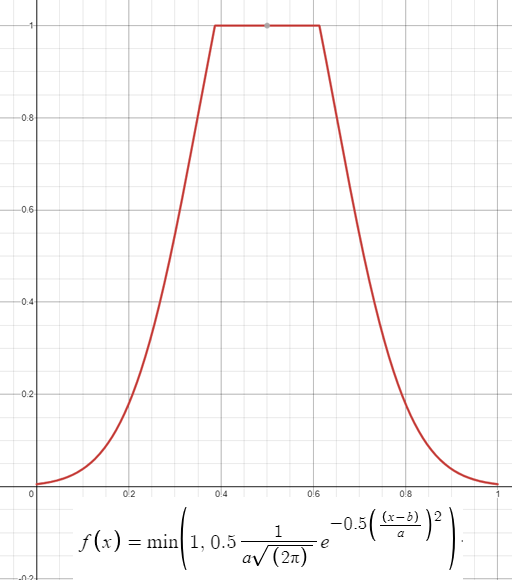
\includegraphics[width=0.32\linewidth]{images/ch20/7a} \hfill
	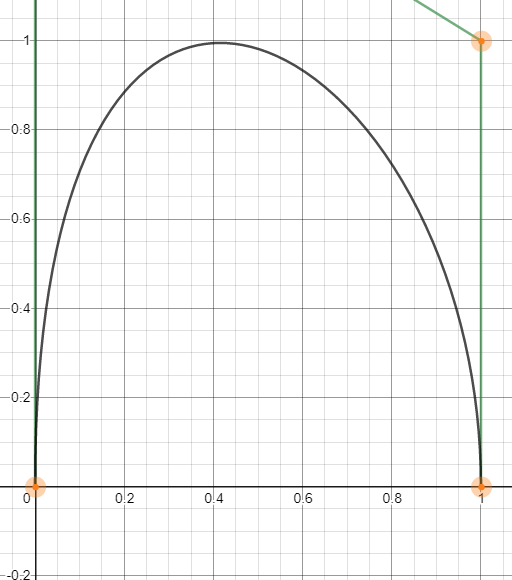
\includegraphics[width=0.32\linewidth]{images/ch20/7b} \hfill
	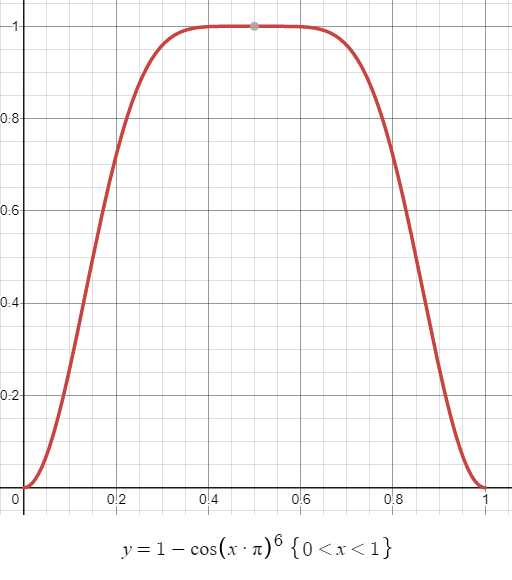
\includegraphics[width=0.32\linewidth]{images/ch20/7c} 
	\caption{Grafici delle tre funzioni interpolabili disponibili negli asset ed utilizzate all'interno del gioco. La scelta di una piuttosto che dell'altra dipende dalla velocità di animazione ricercata nelle due fasi di fade-in e fade-out.}
	\label{fig:f-function}
\end{figure}

\subsubsection{\texttt{C::AABB}}
La componente \cppinline{C::AABB} contiene l'axis-aligned bounding box (AABB) dell'entità necessario al calcolo delle collisioni.
\begin{cpp}
 struct AABB : public fn::Component<AABB> {
     glm::mat2x3 box;
 };
\end{cpp}
Dove \texttt{box} è una matrice le cui colonne sono le coordinate in sistema model dei due estremi (top-left e bottom-right) necessari a definire il box. Si è scelto di utilizzare una matrice per facilitare operazioni di trasformazione delle coordinate.

\subsection{Sistemi}
\marginnote{Tutti system si trovano nel \cppinline{namespace S}.}
In fnGL un system è una qualsiasi struct/class che estende la classe base \cppinline{System}. I sistemi implementano tutte le logiche di gestione, aggiornamento ed eventualmente rendering delle entità, ognuno di essi è applicato a tutte le entità che rispettano i requisiti di componenti del sistema.

\begin{figure}[!htp]
	\centering
	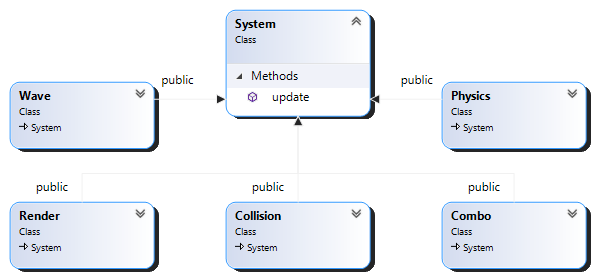
\includegraphics[width=0.95\linewidth]{images/ch20/8}
	\caption{Diagramma UML di tutti sistemu implementate in fnGL.}
	\label{fig:uml-system}
\end{figure}


\begin{exampleBox}
	Il sistema \texttt{S::Physics} gestisce la fisica del gioco relativa al movimento delle entità applicando anche l'{} accelerazione gravitazionale $g$. Per funzionare è necessario:
	\begin{itemize}
		\item la componente \texttt{C::Movement} per calcolare i nuovi vettori velocità applicando $g$;
		\item la componente \texttt{C::Position} per calcolare la nuova posizione.
	\end{itemize}
    Dunque, ad ogni update \texttt{S::Physics} effettua una query per determinare tutti quelle entità con entrambe le componenti\sidenote{Ovvero almeno con la signature \texttt{fn::Sign<C::Position, C::Movement>}.} a applica a ciascuan di esse la sua logica interna di aggiornamento.
\end{exampleBox}


\subsubsection{\texttt{S::Physics}}
Il sistema \cppinline{S::Physics} consente di gestire lo stato fisico delle entità aggiornandone posizione, rotazione, velocità e rendendoli soggetti alla forza gravitazionale. La classe ha anche il compito di eliminare quelle entità che a causa della gravità escono dallo schermo. 

I componenti coinvolti dal sistema sono: \cppinline{C::Position} e \cppinline{C::Movement}.



\subsubsection{\texttt{S::Collision}}
Il sistema \cppinline{S::Collision} si occupa di gestire ciò che avviene quando due oggetti collidono. implementando sia la rilevazione che la risposta alla collisione. I componenti coinvolti dal sistema sono: \cppinline{C::Position}, \cppinline{C::Movement},\\ \cppinline{C::AABB} e \cppinline{C::Fruit}. Nel gioco originale le collisioni non erano gestite in alcun modo.

Le collisioni sono calcolate soltanto per le entità dotate delle precedenti quattro componenti ristrette ulteriormente ai soli frutti interi\sidenote{Per scelta i frutti già tagliati sono intangibili.}. 

\subsubsubsection{Rilevamento delle collisioni}
Il rilevamento delle collisioni avviene utilizzando un approccio ibrido fra OOB e la semplice sfera.
\begin{enumerate}
\item Al momento del caricamento del modello, viene calcolata anche la AABB relativa alle sue coordinate model.
\item Durante il check delle collisioni al AABB viene trasformata in OOB applicando le stesse trasformazioni di modellazione dell'entità al box.
\item A partire da questo nuovo box viene calcolato il raggio della sfera centrato nel centro tangente al suo lato più lungo. Il raggio individua una sfera che sarà utilizzata per la rilevazione.
\end{enumerate}
Si è scelto questo approccio perché semplice e si adatta bene con la quasi totalità dei frutti i quali sono piuttosto tondeggianti.

\subsubsubsection{Risposta alle collisioni}
Quando due frutti collidono, la risposta alla collisione cerca di imitare gli urti elastici della fisica classica. In particolare, si tiene conto delle velocità iniziali e della massa dei frutti per calcolare le velocità relative a seguito dell'impatto. La formula utilizzata è:
\begin{equation}
{\begin{aligned}\mathbf {v} '_{1}&=\mathbf {v} _{1}-{\frac {2m_{2}}{m_{1}+m_{2}}}\ {\frac {\langle \mathbf {v} _{1}-\mathbf {v} _{2},\,\mathbf {x} _{1}-\mathbf {x} _{2}\rangle }{\|\mathbf {x} _{1}-\mathbf {x} _{2}\|^{2}}}\ (\mathbf {x} _{1}-\mathbf {x} _{2}),\\\mathbf {v} '_{2}&=\mathbf {v} _{2}-{\frac {2m_{1}}{m_{1}+m_{2}}}\ {\frac {\langle \mathbf {v} _{2}-\mathbf {v} _{1},\,\mathbf {x} _{2}-\mathbf {x} _{1}\rangle }{\|\mathbf {x} _{2}-\mathbf {x} _{1}\|^{2}}}\ (\mathbf {x} _{2}-\mathbf {x} _{1})\end{aligned}}
\end{equation}
Dove $\mathbf{x}_1$ e $\mathbf{x}_2$ sono i centri dei due oggetti al momento dell'impatto, $\mathbf{v}_1$ e $\mathbf{v}_2$ le velocità dei frutti ed in fine $m_1$ e $m_2$ le loro masse.


\subsubsection{\texttt{S::Wave}}
Il sistema \cppinline{S::Wave} gestisce il lancio di frutti, raggruppandoli in ondate di vario tipo e stabilendo i tempi di lancio. I componenti coinvolti dal sistema sono: \cppinline{C::Position}, \cppinline{C::Movement} e \cppinline{C::Fruit}.

Sono stati implementati quattro ``pattern di lancio":
\marginnote{Tutti i frutti compaiono sempre dal lato basso dello schermo.}
\begin{enumerate}
\item \cppinline{WaveType::RANDOM}: nel quale le componenti dell'entità sono tutte generate casualmente.
\item \cppinline{WaveType::LEFT\_TO\_RIGHT} o \cppinline{WaveType::RIGHT\_TO\_LEFT}: nel quale vengono lanciati in sequenza da sinistra verso destra (o viceversa) più frutti dello stesso tipo.
\item \cppinline{WaveType::SPOT}: nel quale avvengono lanci veloci di frutti dello stesso tipo da posizioni casuali.
\end{enumerate}

\subsubsection{\texttt{S::Combo}}
Il sistema \cppinline{S::Combo} gestisce le combo e i blitz quando si affettano più frutti in rapida successione con un solo swipe.
I componenti coinvolti dal sistema sono \cppinline{C::Sprite} e \cppinline{C::Particle}.


\subsubsection{\texttt{S::Render}}
Il sistema \cppinline{S::Render} disegna le entità tridimensionali e bidimensionali.
I componenti coinvolti dal sistema sono: \cppinline{C::Position} e \cppinline{C::Render} per gli oggetti tridimensionali e \cppinline{C::Sprite} per quelli bidimensionali.

Il rendering avviene in due fasi, prima si disegnano i modelli 3D e poi quelli 2D.




\subsection{Esempio di utilizzo}
\label{ssec:example-ecs}
Creiamo ad esempio tre entità \texttt{e1}, \texttt{e2} ed \texttt{e3} a partire da una istanza di un \cppinline{fn::Database db} nel quale i vari componenti sono già registrati.

\begin{cpp}
 fn::Entity e1 = db.create();
 fn::Entity e2 = db.create();
 fn::Entity e3 = db.create();
\end{cpp}

Le tre entità adesso sono vuote e non hanno associato alcuna componente.

\subsubsection{Set delle componenti}
Una componente può essere aggiunta ad una \cppinline{E::Entity} in due modi tramite il database ed il suo Eid oppure tramite i suoi metodi.
\begin{cpp}[caption={
		Il \texttt{set} può avvenire passando una initialization list, i parametri da inoltrare al costruttore o un oggetto componente.
	}, captionpos=t]
 // set attraverso E::Entity
 e1.set<C::Position>({});   //Costruttore di default
 e1.set<C::Movement>({		//Init list
 	.velocity=glm::vec3(1.5f, 3.6f, 9.1f),
 	.spin=glm::vec3(3.14f, -1.21f, -0.1f),
 });
 e1.set<C::Fruit>({ ... });

 e2.set<C::Position>({}); //Costruttore di default

 // set attraverso fn::Database
 db.set<C::Position>(e3.Eid, {
    .velocity=glm::vec3(1.5f, 3.6f, 9.1f),
    .spin=glm::vec3(3.14f, -1.21f, -0.1f),
 });
\end{cpp}


\subsubsection{Get delle componenti}
Con le stesse modalità del \texttt{set} è anche possibile accedere alle componenti usando la funzione \texttt{get}. Il valore ritornato è sempre un puntatore alla componente. In aggiunta è possibile anche accedere a più componenti insieme, il valore ritornato in questo caso è una \texttt{std::tuple} di puntatori.
\begin{cpp}[caption={
		Utilizzando le funzionalità di un-packing introdotte in c++17 l'utilizzo delle tuple
		risulta molto meno verboso e conveniente. Di fatto l'accesso \enquote{classico} non
		è mai utilizzato.
	}, captionpos=t]
 // get di una singola componente
 auto* p = e1.get<C::Position>();
 
 // get di più componenti classico
 auto t = e1.get<C::Position, C::Movement, C::Fruit>();
 std::get<1>(t)->accelerate(...); //--> C::Movement
 
 // get di più componenti con un-pack (c++17)
 auto [p, m, f] = e1.get<C::Position, C::Movement, C::Fruit>();
 m->accelerate(...); //--> C::Movement
\end{cpp}

\subsubsection{Controllo delle componenti}
Con le stesse modalità del \texttt{get} si può controllare se un'entità ha una o componenti utilizzando il metodo \texttt{has}.
\begin{cpp}
bool a = e1.has<C::Movement, C::Fruit>(); //true 
bool a = e2.has<C::Sprite>(); //false  
\end{cpp}



\subsubsection{Query}
Le query del database possono essere effettuate solo su un oggetto database e in due modi:
\begin{itemize}
\item Usando il metodo \cppinline{Database::having<>} che semplicemente ritorna un vettore\sidenote{questo metodo in realtà non è mai usato nella pratica.} di eid che rispettano la query.
\item Usando il metodo \cppinline{Database::for\_each<>} in combinazione con una funzione lambda che viene applicata ad ogni entità che rispetta la query.
\end{itemize}

\begin{cpp}[caption={
		I vari metodi sono in realtà tutti equivalenti dal punto di vista funzionale, da quello delle performace invece l'iterazione su un sottoinsieme di componenti è sicuramente la scelta migliore.
		\\\\
		Un'ulteriore vantaggio di questo approccio è la possibilità di creare lambda (ad esempio all'interno di eventi di gioco) da applicare alle entità.
	}, captionpos=t]
 // (a) lambda sugli eid
 db.for_each<C::Movement, C::Fruit>([](fn::Eid e){
	// fai qualcosa con e	
 }); 

 // (b) lambda sugli E::Entity
 db.for_each<C::Fruit>([](E::Entity& e){
	// fai qualcosa con e
 }); 
 
 // (c) lambda sui componenti
 db.for_each<C::Position, C::Movement>([](C::Position& p, 
                                          C::Movement& m){
	// fai qualcosa con p ed m
 }); 

 // (c) lambda sui componenti + E::Entity
 db.for_each<C::Sprite>([](E::Entity& e, C::Sprite& s){
	// fai qualcosa con e ed s
 }); 
\end{cpp}





\section{OpenGL}
Questa sezione è dedicata alle classi, funzioni e metodi che sono stati utilizzati per astrarre le primitive di OpenGL combinandole in un API che ne consenta un uso più semplice, componibile e di alto livello.

\subsection{Texture}
La classe \texttt{Texture} gestisce il caricamento, binding e generazione delle texture 2D\sidenote{Le texture 1D o 3D non sono state supportate.} in fnGL. Ogni istanza della classe rappresenta una texture caricata ed è dunque considerata come un asset e gestita dall'AssetManager.
\begin{cpp}
 Texture(const fs::path& texpath, 
         const Texture::Type type = Texture::Type::diffuse, 
         const Texture::Parameteri& parameteri = {});
\end{cpp}
Il costruttore è molto semplice e richiede del caso minimo soltanto il percorso \texttt{texpath} al file immagine contenente la texture; opzionalmente è possibile specificare anche la tipologia di texture (diffuse o specular) e i parametri della texture che saranno passati a \texttt{glTexParameteri}.

L'argomento opzionale \cppinline{Texture::Parameteri parameteri} del costruttore è un alias per \cppinline{std::unordered\_map<GLint, GLint>} utilizzabile per specificare le coppie (key, value) dei parametri. In caso di map vuota verranno utilizzati:
\begin{cpp}
 Texture::Parameteri m_parameteri = {
	{ GL_TEXTURE_WRAP_S, GL_MIRRORED_REPEAT },
	{ GL_TEXTURE_WRAP_T, GL_MIRRORED_REPEAT },
	{ GL_TEXTURE_MIN_FILTER, GL_LINEAR_MIPMAP_LINEAR },
	{ GL_TEXTURE_MAG_FILTER, GL_LINEAR },
 };
\end{cpp} 

\subsubsection{Caricamento e creazione delle texture}
Tutto il lavoro di caricamento delle texture avviene in fase di costruzione dell'oggetto da parte del metodo protected \texttt{Texture::load()} il cui codice è mostrato nel listing sottostante.

\begin{cpp}[caption={Funzione utilizzata per il caricamento, generazione e creazione delle texture in OpenGL.}, captionpos=t]
void Texture::load(){
	stbi_set_flip_vertically_on_load(true);
	
	auto f = this->m_path.string();
	unsigned char* image = stbi_load(f.c_str(), &m_width, 
                                     &m_height, 0, STBI_rgb_alpha);
	if (image == nullptr)
		fn::log::error("[ERRORE] Errore durante il load della \
		                texture {} <image=nullptr>\n", f);
	
	GL_CHECK(glGenTextures(1, &m_id));
	// Eseguo il binding della texture
	GL_CHECK(glBindTexture(GL_TEXTURE_2D, m_id));
	// Setto i parametri 
	for (auto& [key, value] : m_parameteri) {
		GL_CHECK(glTexParameteri(GL_TEXTURE_2D, key, value));
	}
	// Carico i dati della texture
	GL_CHECK(glTexImage2D(GL_TEXTURE_2D, 0, GL_RGBA, m_width,
	                      m_height, 0, GL_RGBA, 
                          GL_UNSIGNED_BYTE, image));
	// Genero eventuali mipmap
	GL_CHECK(glGenerateMipmap(GL_TEXTURE_2D));
	// Pulizia e free
	GL_CHECK(glBindTexture(GL_TEXTURE_2D, 0));
	stbi_image_free(image);
}
\end{cpp}

La prima cosa che ovviamente è necessario fare è caricare i dati detta texture dal file specificato che avviene utilizzando la image-loading library \texttt{stb\_image.h} \cite{STB}. Successivamente, è necessario chiedere ad OpenGL di generare una nuova texture, attivarla eseguendo il binding ed infine settare i parametri. 

Fatto ciò si può procedere a caricare i dati\sidenote{Fino a questo momento i dati si trovano nella memoria ram, con il seguente caricamento verranno trasferiti nella vram.} della texture e a generare eventuali mipmap necessarie.

\subsection{Mesh}
La classe \texttt{Mesh} astrae il concetto di mesh, ovvero rappresenta un reticolo poligonale che definisce un oggetto nello spazio, la rappresentazione avviene mediante vertici, indici e texture. Nei vertici sono contenuti i dati dell'oggetto mentre negli indici contengono l'adjacency information cioè come i vertici sono connessi per formare gli spigoli e le facce della mesh.

\subsubsection{I Vertex}
Per poter creare una mesh è prima necessario definire i vertici. In OpenGL un vertice è molto più di un punto nello spazio, esso può infatti contenere informazioni aggiuntive quali, nomali, coordinate texture, colori, tangenti, bitangenti etc... necessarie rendering avanzato\sidenote{Ad esempio per le luci, ombre, bumps, colori.} degli oggetti. 

L'insieme di tali informazioni insieme al loro ordine e offset all'interno del vertici è detto \textbf{Vertex Layout} che ovviamente può essere dinamico e deve essere specificato ad OpenGL. In fnGL il layout è molto semplice:
\begin{cpp}[caption={Nel vertice si memorizzano la posizione in coordinate model, la normale al vertice per l'illuminazione e le coordinate texure per appunto applicare la texture.}, captionpos=t]
struct Vertex{
	glm::vec3 position;    // Vettore posizione del vertice in coordinate model.
	glm::vec3 normal;      // Vettore normale al vertice
	glm::vec2 texCoords;   // Coordinate del vertice sulla texture
};
\end{cpp}

\subsubsection{Adjacency information}
I vertici da soli non sono sufficienti alla rappresentazione di una mesh e devono essere affiancati dall'{}adjacency information. Si tratta di una serie di indici che specificano terne (o quaterne) di vertici che formano le varie facce\sidenote{In questo modo si evita di memorizzare più volte uno stesso vertici quando si disegnano facce adiacenti ed in oltre è possibile renderizzare sottoinsiemi o definire i lati delle facce a seconda dell'ordine degli indici.} della mesh. 


\subsubsection{Caricamento e creazione delle mesh}
Il caricamento delle mesh avviene con le stesse modalità descritte per le texture nella sezione precedente. 
\begin{enumerate}
\item Si chiede ad OpenGL di generare un \textbf{VAO} (Vertex Array Object) che rappresenterà la nostra mesh sulla GPU.
\item Una volta fatto il bind del VAO si generano i due buffer che conterranno i vertici e gli indici e si procede a caricare tali informazioni:
\begin{itemize}
	\item \textbf{VBO} (Vertex Buffer Object) è il buffer di memoria che conterrà i dati dei vertici.
	\item \textbf{EBO} (Element Buffer Object) è il buffer di memoria che conterrà gli indici.
\end{itemize}
\item Una volta caricati i dati è necessario però specificare il layout dei vertici\sidenote{Ovvero dire ad OpenGL come deve interpretare i dati nel VBO che per ora è un semplice puntatore ad un blocco di byte.\\\\Per l'EBO a meno di specifiche diverse OpenGL assume che il buffer abbia valori innteri su 4Byte.}
La specifica avviene richiamando per ogni attributo del vertice la funzione \texttt{glVertexAttribPointer} specificando dimensione ed offset di partenza.
\end{enumerate}
Il codice esatto non verrà riportato per motivi di spazio.

Un'altro elemento da tenere in considerazione in questa fase è il parametro \texttt{usage} dato insieme al caricamento dei dati. Si tratta di un hint che specifica il pattern di utilizzo atteso di quei buffer per effettuare ottimizzazioni particolari quando ad esempio i dati sono statici o in stream.
\\
In fnGL tutte le mesh sono statiche, una volta caricate non vengono più modificate dunque si è utilizzato il paramtreo \texttt{GL\_STATIC\_DRAW}.


\subsection{Model}
La classe \texttt{Model} astrae il concetto di Modello 3D definito come una composizione di più mesh, solitamente infatti un modello complesso è composto da più mesh e texture. La classe inoltre implementa anche metodi per il caricamente dei modelli utilizzando la libreria ASSIMP.

\marginnote{In realtà, la struttura ad albero è solo logica, tutti i dati si trovano nell'aiScene sottoforma di array, gli altri nodi contengono solo gli indici di accesso a tali dati (ciò consente una maggiore compressione ed evita ripetizioni.)}
La libreria ASSIMP legge il file contenente il modello 3D e lo memorizza internamete in una struttura ad albero; La radice è sempre un nodo del tipo \texttt{aiScene} e contiene tutte le informazioni base e metadati sul modello 3D, la scena può avere dei sottonodi del tipo \texttt{aiNode} che a loro volta possono avere dei sottonodi del tipo \texttt{aiMesh} contenenti le mesh.

\texttt{Model} dunque oltre a comporre più mesh fa da adapter fra la classe \texttt{Mesh} di fnGL e quella di ASSIMP.

\subsection{Shader}
La classe \texttt{Shader} consente di gestire in maniera semplificata alcuni aspetti degli Shader di OpenGL. In particolare:
\begin{enumerate}
	\item Lettura, compilazione e link dei file sorgente \texttt{.glsl} della coppia vertex shader e fragment shader.
	\item Attivazione (e disattivazione) degli shader
	\item Set delle uniform con un'interfaccia polimorfica basata su template.
\end{enumerate}

Gli shader consentono di programmare la pipeline grafica manipolando i dati di vertici e texture. In fnGL sono stati implementati 4 tipi di shader per gestire altrettante esigenze di rappresentazione. 


\subsubsection{Picking shader}
È quello più semplice, il suo scopo è disegnare un oggetto con un unico colore flat; senza luci, ombre o texture. Tale colore identificando univocamente l'oggetto disegnato e potrà essere utilizzato per implementare il picking. 

Il Vertex Shader disegna semplicementge i vertici dell'oggetto secondo la model-view-projection.
\begin{cpp}[caption={Codice sorgente del Vertex Shader. Applica la trasformazione a tutti i vertici del modello.}, captionpos=t]
 #version 330 core
 layout ( location = 0 ) in vec3 position;
 layout ( location = 1 ) in vec3 normal;
 layout ( location = 2 ) in vec2 texCoords;

 uniform mat4 model;
 uniform mat4 view;
 uniform mat4 projection;
 
 void main( )
 {
     gl_Position = projection * view * model * \
 	               vec4( position, 1.0f );
 }
\end{cpp}

Il Fragment Shader disegna con un unico colore (\texttt{r}, \texttt{g}, \texttt{b}, \texttt{a}) l'oggetto.
\begin{cpp}[caption={Codice sorgente del Fragment Shader.}, captionpos=t]
 #version 330
 
 uniform int r;
 uniform int g;
 uniform int b;
 uniform int a;
 
 out vec4 outputF;
 
 void main()
 {
     outputF = vec4(r/255.0, g/255.0, b/255.0, a/255.0);
 }
\end{cpp}




\subsubsection{Blade shader}
È lo shader utilizzato per rappresentare la ``blade" ovvero la lama mostrata quando si scorre con il mouse per tagliare i frutti. 

Il Vertex Shader è simile a quello della sezione precedente, l'unica differenza è il ``forward" delle coordinate texture allo shader successivo in modo che possa utilizzarle per disegnare la lama.
\begin{cpp}[caption={Codice sorgente del Vertex Shader. Applica la trasformazione a tutti i vertici del modello e ritorna le coordinate texture.}, captionpos=t]
 #version 330 core
 layout ( location = 0 ) in vec3 position;
 layout ( location = 1 ) in vec3 normal;
 layout ( location = 2 ) in vec2 texCoords;
 
 out vec2 TexCoords;
 
 uniform mat4 model;
 uniform mat4 view;
 uniform mat4 projection;
 
 void main( )
 {
 	gl_Position = projection * view * model * \ 
 	              vec4( position, 1.0f );
 	TexCoords = texCoords;
 }
\end{cpp}



Il fragment shader utilizza le coordinate texture per determinare il colore dei pixel della mesh. Le coordinate sono interpolate con un sampler2D che dipende dai parametri specificati alla creazione della texture. 
\begin{cpp}[caption={Codice sorgente del Fragment Shader.}, captionpos=t]
 #version 330 core
 
 in vec2 TexCoords;
 out vec4 color;
 
 uniform sampler2D texture_diffuse;
 
 void main( )
 {
 	color = vec4( texture( texture_diffuse, TexCoords ));
 }
\end{cpp}

Le lame implementate hanno texture bicolore e per ottenere bordi netti è necessario utilizzare \texttt{GL\_NEAREST}.

\begin{figure}[!htp]
	\centering
	
\includegraphics[width=0.2\linewidth]{images/ch20/blade0}
	$\quad$
	
\includegraphics[width=0.2\linewidth]{images/ch20/blade1}
	$\quad$
	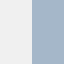
\includegraphics[width=0.2\linewidth]{images/ch20/blade2}
	$\quad$
	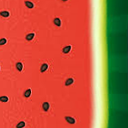
\includegraphics[width=0.2\linewidth]{images/ch20/blade3}
	\caption{Esempio delle tre texture disponibili per le lame. Tutte e quattro derivano da lame realmente esistenti all'interno del gioco.}
	\label{fig:blades}
\end{figure}


\subsubsection{Sprite shader}
Questo shader può essere visto come una semplice estensione di quello usato per disegnare la lama che consente in più di specificare il canale alpha del colore della texture, in questo modo è possibile disegnare oggetti trasparenti.


\subsubsection{Fruit Shader}
Lo shader dedicato al disegno dei frutti e anche quello più complesso dal momento che oltre alle caratteristiche viste in precedenza implementa anche il lighting secondo il modello di riflessione di Phong.


Nel vertex shader oltre alla posizione dei vertici vengono definite anche:
\begin{itemize}
\item La posizione dell'unica sorgente di luce; che deve poi essere convertita in coordinate view. Si tratta di un parametro fisso.
\item Si ricalcolano le normali dei vertici rispetto la model-view.
\end{itemize} 
Queste informazioni sono poi restituite in output allo shader successivo in modo che possa calcolare secondo il modello di Phong le varie componenti della luce.

\begin{cpp}[caption={Codice sorgente del Vertex Shader. Applica la trasformazione a tutti i vertici del modello e ritorna le coordinate texture, posizione della luce e le normali.}, captionpos=t]
#version 330 core
layout (location = 0) in vec3 aPos;
layout (location = 1) in vec3 aNormal;
layout (location = 2) in vec2 aTexCoords;

out vec3 FragPos;
out vec3 Normal;
out vec3 LightPos;

out vec2 TexCoords;

uniform mat4 model;
uniform mat4 view;
uniform mat4 projection;

void main()
{
	// Posizione della luce che illumina la scena
	vec3 lightPos = vec3(0.0f, 30.0f, 30.0f);
	
	gl_Position = projection * view * model * vec4(aPos, 1.0);
	// Calcolo la posizione del fragment
	FragPos = vec3(view * model * vec4(aPos, 1.0));
	// Calcolo le normali
	Normal = mat3(transpose(inverse(view * model))) * aNormal;
	// Coord world -> coord view per la luce
	LightPos = vec3(view * vec4(lightPos, 1.0)); 
	
	TexCoords = aTexCoords;
}
\end{cpp}









Nel fragment shader infine avviene il calcolo della luce e quello del colore della texture, i due valori saranno poi combinato per ottene il colore finale. La luce scelta di base è bianca.
\begin{itemize}
\item \textbf{Luce ambientale}: È la componente ``ambientale" della luce derivante dall'ambiente circostante, gli oggetti infatti non sono mai completamente scuri. È derivata dalla luce di base utilizzando un intensità pari a \texttt{0.4}.

\item \textbf{Luce diffusa}: È la componente diffusiva della luce, che varia a seconda di come i raggi impattano sulla superficie degli oggetti e dall'angolo che si viene a creare fra superfice e sorgente. È derivata dalla luce di base attraverso sua posizione e le normali alle superfici.

\item \textbf{Luce speculare}: È la componente speculare della luce, simula i punti luminosi che si vedono quando la luce riflette su oggetti lucenti. Tale componente varia a seconda dell'angolo fra viwer, superficie e sorgente. Anch'essa è derivata dalla luce di base utilizzando un intensità\sidenote{L'utilizzo di un valore maggiore rende i frutti `plasticosi' e riduce dunque il realismo.} pari a \texttt{0.3} ed un fattore di decay di \texttt{32}.
\end{itemize}

L'unione di queste tre componenti, unite al colore del pixel derivato dalla texture consente di determinare il colore finale dell'oggetto.

\begin{cpp}[caption={Codice sorgente del Fragment shader che implementa l'illuminazione di Phong.}, captionpos=t]
#version 330 core
out vec4 FragColor;

in vec2 TexCoords;
in vec3 FragPos;
in vec3 Normal;
in vec3 LightPos;   // posizione luce in wcoord

uniform sampler2D texture_diffuse;

void main()
{
	// Colore della luce, bianco
	vec3 lightColor = vec3(1.0f, 1.0f, 1.0f);
	
	//::::::::::::::::::::::::::::::::::::::::::::::::
	//::::::  CALCOLO DELLA LUCE AMBIENTALE     :::::: 
	//::::::::::::::::::::::::::::::::::::::::::::::::
	float ambientStrength = 0.4;
	vec3 ambient = ambientStrength * lightColor;    
	
	
	//::::::::::::::::::::::::::::::::::::::::::::::::
	//::::::  CALCOLO DELLA LUCE DIFFUSA        :::::: 
	//::::::::::::::::::::::::::::::::::::::::::::::::
	vec3 norm = normalize(Normal);
	vec3 lightDir = normalize(LightPos - FragPos);
	float diff = max(dot(norm, lightDir), 0.0);
	vec3 diffuse = diff * lightColor;
	
	//::::::::::::::::::::::::::::::::::::::::::::::::
	//::::::  CALCOLO DELLA LUCE SPECULARE      :::::: 
	//::::::::::::::::::::::::::::::::::::::::::::::::
	float specularStrength = 0.3;
	float decay = 32;
	
	// versore alla visione del viewer, nel  view-space
	// il viewer sta sempre in (0,0,0)
	vec3 viewDir = normalize(-FragPos); 
	vec3 reflectDir = reflect(-lightDir, norm);  
	float spec = pow(max(dot(viewDir, reflectDir), 0.0), decay);
	vec3 specular = specularStrength * spec * lightColor; 
	
	
	// Combino i risultati con il colore della texture
	vec3 objectColor = (texture( texture_diffuse, TexCoords)).xyz;
	vec3 result = (ambient + diffuse + specular) * objectColor;
	FragColor = vec4(result, 1.0);
}
\end{cpp}
%\setchapterpreamble[u]{\margintoc}
\chapter{Implementazione GPU}

\begin{chap-intro}
	In questo capitolo si descriverà l'implementazione effettuata del radix-sort in ambiente CUDA analizzando il funzionamento dei vari kernel utilizzati. Per avere un confronto con la CPU verrà poi illustrata una implementazione dello stesso algoritmo in ambiente OpenMP. Successivamente verranno mostrati i risultati di test, prove e Benchmark fra le soluzioni proposte e quelli presenti nella libreria \texttt{CUB} \cite{CUB}.
\end{chap-intro}


\section{Implementazione GPU}
In questa sezione verrà da prima decritto il funzionamento dell' applicazione proposta mostrandone l'interfaccia ed un esempio di utilizzo, successivamente i vari kernel utilizzati verranno descritti più nel dettaglio.

\subsection{Compilazione ed esecuzione}
Il progetto è stato strutturato in più cartelle, le principali sono:
\begin{itemize}
\item La cartella \texttt{/include} contiene gli header delle funzioni nel formati \texttt{.h} (per i C++) o \texttt{.cuh} (per i CUDA kernel).
\item La cartella \texttt{/src} contiene i sorgenti che essi siano \texttt{.cpp} o \texttt{.cu}.
\item La cartella \texttt{/app} contiene l'entry point all'applicazione dove si effettua un benchmark del radix-sort implementato.
\end{itemize}

Per la compilazione è sufficiente posizionarsi nella root principale ed utilizzare il comando:

\begin{lstlisting}[style=console, caption={Comando per compilare il progetto. L'eseguibile prodotto è chiamato \texttt{app} e posizionato nella sotto-cartella \texttt{/bin}.}, label={compile-command}]
> nvcc -std=c++11 -O3 -Xptxas -O3 -Xcompiler -O3 -Iinclude 
       app/main.cpp src/radix_sort.cu src/scan.cu -o bin/app 
\end{lstlisting}

L'eseguibile prodotto è chiamato \texttt{app} e posizionato nella sotto-cartella \texttt{/bin}. Per eseguirlo è sufficiente utilizare il comando \texttt{./bin/app}. L'output prodotto sarà:

\begin{lstlisting}[style=console, caption={Esecuzione ed output orodotto dell'applicativo. L'array generato ha valori uniformemente distribuiti fra {$[0, 2^{32}-1]$} ed i tempi (misurati in microsecondi) includono il trasferimento di memoria fra host e device.}, label={compile-command}]
> ./bin/app

  ::::::::::::::::::::::::::::::::::::::::::::
  ::::      Benchmark radix-sort GPU      ::::
  ::::::::::::::::::::::::::::::::::::::::::::
   Ordinamento di unsigned int a 32b        
    - Unif. distribuiti in [0, 2<<32-1]     
    - Array di dimensioni crescenti 
 
   ARRAY SIZE         TEMPO (us)     CPU==GPU  
       1024 (2**10)         2831      uguali 
       2048 (2**11)         4206      uguali 
       4096 (2**12)         7168      uguali  
       8192 (2**13)        13211      uguali  
      16384 (2**14)        25282      uguali 
      32768 (2**15)        27708      uguali 
      65536 (2**16)        36380      uguali 
     131072 (2**17)        37964      uguali  
     262144 (2**18)        38389      uguali 
     524288 (2**19)        39060      uguali 
    1048576 (2**20)        41242      uguali 
    2097152 (2**21)        44165      uguali 
    4194304 (2**22)        50840      uguali 
    8388608 (2**23)        99571      uguali 
   16777216 (2**24)       161666      uguali 
   33554432 (2**25)       320561      uguali 
   67108864 (2**26)       605680      uguali 
  134217728 (2**27)      1217086      uguali 
  268435456 (2**28)      2408928      uguali 
\end{lstlisting}

\subsection{API ed esempio}
L'implementazione è definita dell'header cuda \texttt{radix\_sort.h}.
\begin{cpp}
void RadixSortGPU::sort(unsigned int* first, unsigned int* last);
\end{cpp}
L'interfaccia è simile a \texttt{std::sort} della standard template library:
\begin{itemize}
\item La funzione si trova nel namespace \texttt{RadixSortGPU};
\item Richiede du parametri \texttt{first} e \texttt{last} rappresentano gli estremi del range di elementi dell'\textit{array host} ordinare;
\item Lavora in-place sovrascrivendo l'input.
\end{itemize} 

\subsubsection{Esempio di utilizzo}
Di seguito un esempio di utilizzo del radix sort per l'ordinamento di un piccolo array da 14 elementi.
\begin{cpp}[caption={%
		Esempio di funzionamento dell'implementazione del radix-sort per ordinare un array utilizzando la GPU.
		L'array in input \texttt{array\_GPU} si trova sull'host ha dimensione 14 ed è stato copiato in \texttt{array\_CPU} per la verifica di correttezza su CPU.
		\\
		L'interfaccia ed il funzionamento di \texttt{RadixSortGPU::sort(*)} è simile a \texttt{std::sort(*)} della STD del C++.
	},%
 label={example-code}, captionpos=t]
#include <iostream>
#include "radix_sort.cuh"

typedef unsigned int uint;
int main(){
	uint array_GPU[] = {5, 7, 4, 2, 8, 6, 1, 9, 0, 3, 2, 3, 1, 3}; 
	constexpr int N = sizeof(array_GPU)/sizeof(uint);
	uint array_CPU[N];
	std::copy(array_GPU, array_GPU + N, array_CPU);
	
	std::cout << "Array originale:  ";
	for (auto a : array_GPU) std::cout << a << " ";
	
	// Array ordinato su GPU
	RadixSortGPU::sort(array_GPU, array_GPU + N);    
	std::cout << "\nordinato con GPU: ";
	for (auto a : array_GPU) std::cout << a << " ";
	
	// Array ordinato su CPU
	std::sort(array_CPU, array_CPU + N);             
	std::cout << "\nordinato con CPU: ";
	for (auto a : array_CPU) std::cout << a << " ";
	std::cout << '\n';
	
	return 0;
}
\end{cpp}

\bigskip
\textbf{Output}
\begin{lstlisting}[style=console, caption={Output dell'esempio. Come è possibile vedere l'output dell'algoritmo su CPU coincide con quello prodotto sulla GPU.}, label={execution}]
> ./example
  Array originale:  5 7 4 2 8 6 1 9 0 3 2 3 1 3
  ordinato con GPU: 0 1 1 2 2 3 3 3 4 5 6 7 8 9
  ordinato con CPU: 0 1 1 2 2 3 3 3 4 5 6 7 8 9
\end{lstlisting}


\subsection{Dettagli implememtativi}
L'implementazione effettuata segue il paper \cite{Satish2009} tuttavia a seguito di alcuni test si è preferito modificare alcuni parametri, in particolare:
\marginnote[*+1]{
	Utilizzando $b=256$ l'ordinamento è effettuato un byte alla volta, per un intero senza segno su una macchina classica sono dunque necessari 4 counting-sort.
}
\begin{itemize}
	\item Dimensione della base $b$: È stata utilizzata una base $b=256$ invece di $b=16$. In questo modo gli istogrammi sono più grandi (è richiesta molta più shared memory) ma si dimezza il numero di iterazioni del counting sort ed il trasferimento con la memoria globale e gli accessiad essa.
	\item Dimensione del tile: È stato utilizzato un tile di dimensioni $16.384$ (dato l'istogramma più grande). In questo modo il numero di blocchi si riduce ed ogni thread gestisce $64$ elementi.
\end{itemize}


\subsubsection{RadixSortGPU::sort}
La procedura \cppinline{RadixSortGPU::sort(*)} mostrata nel listing \rref{sort-code} è la funzione principale dell'implementazione. Qui non si effettuano ancora chiamate dirette ai kernel CUDA.
\begin{enumerate}
\item Calcolo del numero di blocchi \texttt{P};
\item Allocazione della memoria e trasferimento dell'array sul device;
\item Ordinamento attraverso 4 chiamante di \texttt{partial\_sort}\sidenote{Ovvero viene effettuato un counting sort per ognununa delle 4 radici.}. %
%Dopo ogni ordinamento parziale la copia fra buffer e array è evitata scambiando i puntatori sul device.
\item Trasferimento dell'array ordinato sull'host e deallocazione della memoria usata.
\end{enumerate}

\begin{cpp}[caption={%
		Estratto del codice della procedura principale ordinamento.
	},%
	label={sort-code}, captionpos=t]
void RadixSortGPU::sort(uint* first, uint* last){
	const size_t N = std::distance(first, last);
	const size_t P = (N + TILE_SIZE - 1) / TILE_SIZE;
	
	// Alloco la memoria necessaria all'ordinamento
	uint* d_array = nullptr;
	cuda::malloc(d_array, N*sizeof(uint));
	uint* d_tmp = nullptr;
	cuda::malloc(d_tmp, N*sizeof(uint));
	uint* d_hist = nullptr;
	cuda::malloc(d_hist, P*BUCKETS_COUNT*sizeof(uint));
	
	// Trasferisco l'array sul device
	cuda::memcpy(d_array, first, N*sizeof(uint), 
	             cuda::memcpyKind::HostToDevice);
	
	// Effettuo l'ordinamento...
	partial_sort<0>(d_array, d_tmp, N, d_hist); 
	std::swap(d_array, d_tmp);
	partial_sort<1>(d_array, d_tmp, N, d_hist); 
	std::swap(d_array, d_tmp);
	partial_sort<2>(d_array, d_tmp, N, d_hist); 
	std::swap(d_array, d_tmp);
	partial_sort<3>(d_array, d_tmp, N, d_hist); 
	std::swap(d_array, d_tmp);

	// Trasferisco l'array ordinato all'host
	cuda::memcpy(first, d_array, N*sizeof(uint), 
	             cuda::memcpyKind::DeviceToHost);
	
	// Libero la memoria allocata
	cuda::free(d_array);
	cuda::free(d_tmp);
	cuda::free(d_hist);
}
\end{cpp}

\subsubsection{RadixSortGPU::partial\_sort<>}
La procedura \cppinline{RadixSortGPU::partial_sort<>(*)} mostrata nel listing \rref{partial-code} implementa il counting-sort eseguendo sequenzialmente le 3 macro-fasi richiamando gli appositi kernel. L'ordinamento avviene rispetto all'indice della radice \texttt{RADIX} fornito nel template.

\begin{cpp}[caption={%
		Estratto del codice della procedura partial di ordinamento.
	},%
	label={partial-code}, captionpos=t]
template<uint RADIX>
void RadixSortGPU::partial_sort(uint* d_array, uint* d_tmp, 
                                size_t N, uint* d_hist){
	const size_t P = (N + TILE_SIZE - 1) / TILE_SIZE; 
	
	// Ogni blocco calcola il suo istogramma di TILE_SIZE elementi
	RadixSortGPU::tile_histograms<RADIX>(d_array, N, d_hist);
	
	// Effettuo la scan dell'istogramma
	RadixSortGPU::prefix_scan(d_hist, P*BUCKETS_COUNT);
	
	// Distribuisco gli elementi 
	RadixSortGPU::rank_n_permute<RADIX>(d_array, d_tmp, N, d_hist);
}
\end{cpp}


\subsubsection{Estrazione della radice}
Tramite la funzione \cppinline{RadixSortGPU::digit<>(*)} mostrata nel listing \rref{digit-code} viene estratta la \texttt{RADIX}-esima radice da un intero. L'operazione di estrazione avviene attraverso semplici operazioni bitwise.
\begin{cpp}[caption={%
		Estratto del codice della procedura partial di ordinamento.
		\texttt{RADIX\_SIZE} è $b$. 
	},%
	label={digit-code}, captionpos=t]
template <uint RADIX>
__device__ inline constexpr uint digit(const uint value){
	return (value >> RADIX*RADIX_SIZE) & ((1 << RADIX_SIZE) - 1);
}
\end{cpp}


\subsection{Dettagli implememtativi Kernel}
In questa sezione verranno illustrati i kernel tramite i quali sono implementate le tre macro-fasi del counting sort. In particolare, la prima fase di \texttt{histogram} e l'ultima di \texttt{rank-and-permute} utilizzano due tipologie di kernel, a seconda se l'ordinamento è stabile o meno.

Mantenere la proprietà di stabilità rende i kernel più lenti\sidenote{A causa dei pattern di accesso alla memoria. Infatti ogni thread del blocco deve \textit{accedere ordinatamente} agli indici dell'array da ordinare.} ma non è necessario farlo per la prima radice che si sta ordinando. La prima iterazione può quindi essere effettuata con kernel non-stabili mentre le restanti devono essere effettuate con kernel stabili.


\subsubsection{Kernel - {histogram} (non-stabile)}
Il kernel \cppinline{histogram_kernel_unstable<>(*)} mostrato nel listing \rref{histogram-kernel-unstable-code} utilizza \texttt{blockDim.x} thread per calcolare l'istogramma parziale rispetto la radice \texttt{RADIX} di ciascun blocco e lo memorizza nella giusta locazione della global memory; l'{}istogramma è calcolato in maniera non-stabile.

\medskip
\noindent
\textbf{\color{black!65!white}\small\HeadingsFont{Parametri}}\\
I parametri del kernel sono:

\begin{table}[!htp]
\begin{tabular}{rcp{6.5cm}}
\cppinline{uint RADIX} &-& indice della radice da estrarre (LSD); \\
\cppinline{uint *d_in} &-& puntatore al device array di input per il quale si vuole calcolare l'istogramma; \\
\cppinline{size_t N}  &-& numero di elementi in input; \\
\cppinline{uint *d_hist} &-& puntatore al device array di output\sidenote{Corrisponde alla matrice $\m{H}$ linearizzata.} dove memorizzare gli istogrammi parziali.
\end{tabular}
\end{table}

\noindent
\textbf{\color{black!65!white}\small\HeadingsFont{Descrizione}}\\
Il kernel deve essere invocato con \texttt{blockDim.x = 256} in quanto ogni thread è responsabile di un bin dell'istogramma. %
\marginnote{%
Per semplificare la fase di scan, \texttt{d\_hist} è memorizzato in maniera \textit{column-major} in questo modo la scansione può essere applicato direttamente sulla sua linearizzazione.
}%
Dopo l'inizializzazione, ogni thread calcola la posizione e gli offset su \texttt{d\_in} estrae la radice e aumenta in maniera atomica il relativo bin; successivamente ogni thread salva il valore del suo bin in \texttt{d\_hist}.

\begin{cpp}[caption={%
		Estratto del codice della procedura partial di ordinamento.
		Il numero di buckets \texttt{BUCKETS\_COUNT} equivale alla base $b$ di numerazione. 
	},%
	label={histogram-kernel-unstable-code}, captionpos=t]
template <uint RADIX> __global__ 
void histogram_kernel_unstable(uint *d_in, size_t N, uint *d_hist){   
	__shared__ uint temp[RadixSortGPU::BUCKETS_COUNT];
	
	temp[threadIdx.x] = 0;
	__syncthreads();
	
	int i = threadIdx.x + blockIdx.x*blockDim.x;
	const int offset = blockDim.x * gridDim.x;
	while (i < N){
		atomicAdd(&temp[digit<RADIX>(d_in[i])], 1);
		i += offset;
	}
	__syncthreads();
	
	d_hist[blockIdx.x + threadIdx.x*gridDim.x] = temp[threadIdx.x];
}
\end{cpp}
Ogni blocco processa porzioni \textit{non contigue} di 256 elementi alla volta fin tanto che l'array non termina. L'istogramma parziale del blocco sarà in ogni caso costruito su \texttt{TILE\_SIZE} elementi ma essendoci dei \enquote{salti} fra le porzioni si perde la stabilità durante il successivo calcolo degli offset. 

\subsubsection{Kernel - {histogram} (stabile)}
Il kernel \cppinline{histogram_kernel<>(*)} mostrato nel listing \rref{histogram-kernel-code} mantenendo l'ordine di assegnazione\sidenote{Dunque il $k$-esimo blocco con id:$k$ riceverà gli elementi fra [$k$\texttt{TILE\_SIZE}, $(k+1)$\texttt{TILE\_SIZE}[ } delle porzioni di tile ai thread è stabile.

\medskip
\noindent
\textbf{\color{black!65!white}\small\HeadingsFont{Parametri}}\\
I parametri del kernel sono:

\begin{compactcenter}
	\begin{tabular}{rcp{6.5cm}}
		\cppinline{uint RADIX} &-& indice della radice da estrarre (LSD); \\
		\cppinline{uint *d_in} &-& puntatore al device array di input per il quale si vuole calcolare l'istogramma; \\
		\cppinline{size_t N}  &-& numero di elementi in input; \\
		\cppinline{uint *d_hist} &-& puntatore al device array di output dove memorizzare gli istogrammi parziali.
	\end{tabular}
\end{compactcenter}

\noindent
\textbf{\color{black!65!white}\small\HeadingsFont{Descrizione}}\\
Il funzionamento generale di questo kernel è simile al precedente, anche in questo caso deve essere invocato con \texttt{blockDim.x = 256} in quanto ogni thread è responsabile di un bin dell'istogramma. La differenza sta nel calcolo degli indici e degli offset, ogni blocco riceve ordinatamente i tile di \texttt{TILE\_SIZE} ed i thread al loro interno ne calcoleranno gli istogrammi.

\begin{cpp}[caption={%
		Estratto del codice della procedura partial di ordinamento.
		Il numero di buckets \texttt{BUCKETS\_COUNT} equivale alla base $b$ di numerazione. 
	},%
	label={histogram-kernel-code}, captionpos=t]
template <uint RADIX> __global__ 
void histogram_kernel(uint *d_in, size_t N, uint *d_hist){   
	__shared__ uint temp[RadixSortGPU::BUCKETS_COUNT];
	
	temp[threadIdx.x] = 0;
	__syncthreads();
	
	const int EPB = N / gridDim.x;
	
	const int i = threadIdx.x + blockIdx.x*EPB;
	const int offset = blockDim.x;
	int j = 0;
	
	while (j < EPB && i + j < N){
		atomicAdd(&temp[digit<RADIX>(d_in[i+j])], 1);
		j += offset;
	}
	__syncthreads();
	
	d_hist[blockIdx.x + threadIdx.x*gridDim.x] = temp[threadIdx.x];
}
\end{cpp}

\subsubsection{Invocazione dei kernel histogram}
Nel seguente listing è in fine mostrato come sono invocati i kernel. Il numero di thread per blocco equivale al numero di buckets \texttt{BUCKETS\_COUNT}=$b$ nell'istogramma, mentre il numero di blocchi è calcolato dinamicamente a partire dal numero di elementi e dal \texttt{TILE\_SIZE}.
Se la radice che si sta ordinando è la prima allora viene richiamata la versione non stabile, altrimenti quella stabile.
\begin{figure*}[!hpt]
\begin{cpp}
template <uint RADIX>
void RadixSortGPU::histogram(uint *d_in, size_t N, uint* d_hist){
	const size_t P = (N + TILE_SIZE - 1) / TILE_SIZE;
	if(RADIX == 0)
		histogram_kernel_unstable<RADIX><<<P, BUCKETS_COUNT>>>(d_in, N, d_hist);
	else
		histogram_kernel<RADIX><<<P, BUCKETS_COUNT>>>(d_in, N, d_hist);
}
\end{cpp}
\end{figure*}


\subsubsection{Kernel - {scan}}
L'exclusive prefix sum (scan) è un \enquote{building block} per molti algoritmi paralleli tra cui l'ordinamento e la costruzione di strutture di dati. Si tratta dunque di una primitiva che non necessita di re-implementazioni, nel paper in esame infatti per tale operazione si ricorre alla libreria CUDPP\sidenote{CUDA Data Parallel Primitives Library. \url{http://cudpp.github.io/}
\\
Il radix-sort proposto nel paper sarà poi successivamente aggiunto a tale collezione di primitive.
}. 

Il principale problema della libreria CUDPP è che ha delle limitazioni dulla dimensione massima degli array di input, in particolare nel caso di scan la dimensione massima supportata è $67.107.840$ elementi ($\approx 2^{26}$). Per ordinare array di dimensioni maggiori, nel lavoro svolto, si è preferito utilizzare\sidenote{Alla quale sono state solamente effettuate alcune modifiche all'interfaccia delle funzioni richiamate.} l'implementazione di \textsc{matt dean} \cite{mattdean1} disponibile su github a sua volta basata sul paper \cite{harris2007parallel} di NVIDIA, autore \textsc{mark harris} pubblicato nella collezione di GPU Gems 3 da NVIDIA. 




\subsubsection{Kernel - {rank-and-permute} (non stabile)}
Il kernel \cppinline{rank_n_permute_kernel_unstable<>(*)} mostrato nel listing \rref{histogram-kernel-code} implementa la terza macro-fase del counting-sort in maniera non stabile. La struttura è simile al kernel dell'istogramma, ogni blocco gestisce un istogramma parziale, lo carica in memoria e iterando sul vettore originale lo sfrutta per calcolare gli offset e le posizioni finali.

\medskip
\noindent
\textbf{\color{black!65!white}\small\HeadingsFont{Parametri}}\\
I parametri del kernel sono:

\begin{compactcenter}
	\begin{tabular}{rcp{6.5cm}}
		\cppinline{uint RADIX} &-& indice della radice da estrarre (LSD); \\
		\cppinline{uint *d_in} &-& puntatore al device array di input; \\
		\cppinline{uint *d_out} &-& puntatore al device array di output; \\
		\cppinline{size_t N}  &-& numero di elementi in input e output; \\
		\cppinline{uint *d_hist} &-& puntatore al device array dove leggere gli istogrammi parziali.
	\end{tabular}
\end{compactcenter}

\noindent
\textbf{\color{black!65!white}\small\HeadingsFont{Descrizione}}\\
Anche in questo caso deve essere invocato con \texttt{blockDim.x = 256} in quanto ogni thread è responsabile di un bin dell'istogramma. Ogni thread del blocco scorre la sua porzione di array estrae la radice dai suoi valori e la usa per calcolare la posizione finale di quell'elemento, una volta calcolata tale posizione il bin relativo a quella radice può essere incrementato \textit{atomicamente}.

\begin{cpp}[caption={%
		Estratto del codice della procedura partial di ordinamento.
		\texttt{RADIX\_SIZE} è $b$. 
	},%
	label={rank-and-permute-unstable-code}, captionpos=t]
template<uint RADIX> __global__ 
void rank_n_permute_kernel_unstable(uint* d_in, uint* d_out, 
                                    size_t N, uint* d_hist){
	__shared__ uint temp[RadixSortGPU::BUCKETS_COUNT];
	
	temp[threadIdx.x] = d_hist[blockIdx.x + threadIdx.x*gridDim.x];
	__syncthreads();
	
	int i = threadIdx.x + blockIdx.x * blockDim.x;
	const int offset = blockDim.x * gridDim.x;
	while (i < N){
		uint new_index = atomicAdd(&temp[digit<RADIX>(d_in[i])], 1);
		d_out[new_index] = d_in[i];
		i += offset;
	}
}
\end{cpp}

\subsubsection{Kernel - {rank-and-permute} (stabile)}
Il kernel \cppinline{rank_n_permute_kernel<>(*)} mostrato nel listing \rref{histogram-kernel-code} implementa stabilmente la terza macro-fase del counting-sort. La struttura è simile al kernel dell'istogramma, con la differenza che ogni blocco è in grado di gestire più di un istogramma parziale.

\medskip
\noindent
\textbf{\color{black!65!white}\small\HeadingsFont{Parametri}}\\
I parametri del kernel sono:

\begin{compactcenter}
	\begin{tabular}{rcp{6.5cm}}
		\cppinline{uint RADIX} &-& indice della radice da estrarre (LSD); \\
		\cppinline{uint *d_in} &-& puntatore al device array di input; \\
		\cppinline{uint *d_out} &-& puntatore al device array di output; \\
		\cppinline{size_t N}  &-& numero di elementi in input e output; \\
		\cppinline{uint *d_hist} &-& puntatore al device array dove leggere gli istogrammi parziali.
	\end{tabular}
\end{compactcenter}

\noindent
\textbf{\color{black!65!white}\small\HeadingsFont{Descrizione}}\\
Gli istogrammi sono caricati in nella shared memory e gestiti ognuno da un thread responsabile di tutti i suoi 256 bin. Ogni thread del blocco scorre la sua porzione di array estrae la radice dai suoi valori e la usa per calcolare la posizione finale di quell'elemento, una volta calcolata tale posizione il bin relativo a quella radice può essere incrementato senza bisogno di operazioni atomiche.

\begin{cpp}[caption={%
		Estratto del codice della procedura partial di ordinamento.
		\texttt{RADIX\_SIZE} è $b$. 
	},%
	label={rank-and-permute-code}, captionpos=t]
template<uint RADIX> __global__ 
void rank_n_permute_kernel(uint* d_in, uint* d_out, size_t N, 
                           uint* d_hist){
	extern __shared__ uint temp[];
	for(int i = 0; i < BUCKETS_COUNT; i++){
		auto ix = blockIdx.x*blockDim.x + threadIdx.x +
		          i * gridDim.x * blockDim.x
		temp[threadIdx.x*BUCKETS_COUNT + i] = d_hist[ix];
	}
	
	const int EPB = N / gridDim.x;
	const int EPT = (EPB + blockDim.x - 1) / blockDim.x;
	
	const int i = threadIdx.x*EPT + blockIdx.x*EPB;
	for(int j = 0; j < EPT && i+j < N; j++){
		const int pos =  digit<RADIX>(d_in[i+j]) + 
		                 threadIdx.x*BUCKETS_COUNT;
		d_out[temp[pos]++] = d_in[i+j];
	}
}
\end{cpp}


\section{Implementazione CPU}
\marginnote{
	L'implementazione CPU è in realtà molto più \enquote{funzionale} rispetto a quella GPU perchè nasce da esigenze specifiche di implementazione all'interno del DBMS SADAS. Ad esempio è possibile ordinare interi, float e stringhe, si può specificare tramite template il numero di radici e la loro dimensione (perchè spesso i valori da ordinare sono su 1/2/3 Byte) oppure è possibile specificare come estrarre le radici quando si ordina (per i float e stringhe).
}
Per avere un confronto sul guadagno di performance del radix-sort su GPU è stata implementata, seguendo le stesse idee della sezione \rref{ssec:194401} una variante parallela di radix-sort per CPU utilizzando OpenMP.

\subsection{API ed esempio}
Anche in questo caso l'interfaccia del sort è simile a \texttt{std::sort} della standard template library:

\begin{cpp}
template <unsigned int RADIX_SIZE = 8, unsigned int KEYSIZE = 0>
class RadixSort{
	...
	template <class RandomAccessIterator, class RadixAccess>
	static void sort(RandomAccessIterator first, 
	                 RandomAccessIterator last, 
	                 RadixAccess access, 
	                 Algorithm algorithm = Algorithm::LSD);	
	...
}
\end{cpp}
Grazie ai template la funzione è generica in grado di ordinare qualsiasi struttura dati che rispetti i requisiti di RandomAccessIterator della STD.

\subsubsection{Esempio di utilizzo}
Di seguito un esempio di utilizzo del radix sort per l'ordinamento di un piccolo array da 14 elementi.
\begin{cpp}[caption={%
		Esempio di funzionamento dell'implementazione del radix-sort per ordinare un array utilizzando la CPU.
		L'array in input \texttt{array\_RDX} ha dimensione 14 ed è stato copiato in \texttt{array\_STD} per la verifica di correttezza.
		\\
		Interfaccia e funzionamento di \texttt{RadixSort<>::sort(*)} sono simili a \texttt{std::sort(*)} della STD del C++.
		\\\\
		Nelle parentesi angolari della classe (\texttt{RadixSort<>}) è possibile specificare la dimensione in bit della radice ed
		il numero di radici da utilizzare per l'ordinamento. In questo esempio, la chiamata  
		\texttt{RadixSort<4,1>::sort(*)} avrebbe consentito di risparmiare 3 iterazioni inutili e usare meno bins.
	},%
	label={example-2-code}, captionpos=t]
#include <iostream>
#include "RadixSort.h"

typedef unsigned int uint;
int main(){
	uint array_RDX[] = {5, 7, 4, 2, 8, 6, 1, 9, 0, 3, 2, 3, 1, 3}; 
	constexpr int N = sizeof(array_RDX)/sizeof(uint);
	uint array_STD[N];
	std::copy(array_RDX, array_RDX + N, array_STD);
	
	std::cout << "Array originale:  ";
	for (auto a : array_RDX) std::cout << a << " ";
	
	// Array ordinato con RadixSort<>::sort(*)
	RadixSort<>::sort(array_RDX, array_RDX + N);    
	std::cout << "\nordinato con RDX: ";
	for (auto a : array_RDX) std::cout << a << " ";
	
	// Array ordinato con std::sort(*)
	std::sort(array_STD, array_STD + N);             
	std::cout << "\nordinato con STD: ";
	for (auto a : array_STD) std::cout << a << " ";
	std::cout << '\n';
	
	return 0;
}
\end{cpp}

\bigskip
\textbf{Output}
\begin{lstlisting}[style=console, caption={Output dell'esempio. Come è possibile vedere gli output coincidono.}, label={execution-2}]
> ./example
Array originale:  5 7 4 2 8 6 1 9 0 3 2 3 1 3
ordinato con RDX: 0 1 1 2 2 3 3 3 4 5 6 7 8 9
ordinato con STD: 0 1 1 2 2 3 3 3 4 5 6 7 8 9
\end{lstlisting}






\subsection{Dettagli implementativi}
In questa sezione è semplicemnete listato il codice relativo all' implementazione parallela del radix-sort LSD su CPU tramite la libreria OpenMP. 

In particolare verranno prima mostrate le funzioni relative alle tre macro-fasi del counting-sort e successivamente la procedura principale \texttt{LSD\_radix\_sort}.


\subsubsection{Histogram}
\begin{cpp}
template <unsigned int BUCKETS, typename dtype, class RadixAccess>
static void compute_hist(const dtype* array, const size_t N, 
                         unsigned int* hist,
                         const RadixAccess& access, 
                         const unsigned int idx){
	#pragma omp parallel for schedule(static)
	for(unsigned int i = 0; i < N; i++){
		const unsigned int dgt = access(array[i], idx);
		++hist[dgt + omp_get_thread_num() * BUCKETS]; 
	}
}
\end{cpp}

\medskip
\subsubsection{Scan}
\begin{cpp}
template <int BUCKETS>
static void prefix_sum(unsigned int* hist){
	unsigned int sum = 0;
	for(int i = 0; i < BUCKETS; i++)
	for(int j = 0; j < omp_get_max_threads(); j++){
		const unsigned int tmp = hist[i + j * BUCKETS];
		hist[i + j * BUCKETS] = sum;
		sum += tmp;
	}   
}
\end{cpp}

\medskip
\subsubsection{Rank-and-Permute}
\begin{cpp}
template <unsigned int BUCKETS, typename dtype, class RadixAccess>
static void integer_sort(dtype* array, dtype* tmp, const size_t N, 
                         unsigned int* hist, 
                         const RadixAccess& access, 
                         const unsigned int idx){
	#pragma omp parallel for schedule(static)
	for(unsigned int i = 0; i < N; i++){
		const unsigned int pos = access(array[i], idx) + omp_get_thread_num() * BUCKETS;
		tmp[hist[pos]] = array[i];
		++hist[pos];
	}
}	
\end{cpp}

\medskip
\noindent
\textbf{\small\HeadingsFont{Algoritmo completo}}\vspace{-0.5cm}
\begin{figure*}[!hpt]
\begin{cpp}
template <class RandomAccessIterator, class RadixAccess, 
typename dtype = typename std::iterator_traits<RandomAccessIterator>::value_type>
static void LSD_radix_sort(const RandomAccessIterator first, 
const RandomAccessIterator last, const RadixAccess& access){
	// Numero di iterazioni necessarie, una per radice                       
	constexpr int runs = KEYSIZE > 0 ? KEYSIZE : (sizeof(dtype)*8 + RADIX_SIZE - 1)/RADIX_SIZE;
	// Numero di bucket per radice 
	constexpr const unsigned int BUCKETS = (1 << RADIX_SIZE);  
	// Numero totale di bucket (per la parallelizzazione)        
	const unsigned int hBins = omp_get_max_threads() * BUCKETS;        
	//Trasformo gli iteratori in un array C-Style
	auto* array = &(*first);
\end{cpp}
\end{figure*}
\begin{figure*}[!hpt]
\begin{cpp}	
	const size_t N = std::distance(first, last);
	
	//Pre-alloco la memoria ausiliaria per il calcolo dell'istogramma e vettore di appoggio
	unsigned int hist[hBins];           // Ogni thread calcolerà il suo istogramma parziale.
	auto* tmp = new dtype[N];           // Array di appoggio per l'integer-sort.
	
	// Avvio algoritmo di ordinamento
	int iter = 0;
	for(int i = 0; i < runs; i++){
		memset(hist, 0, sizeof(unsigned int)*hBins);
		
		// Fase 1: Calcolo dell'istogramma dell'i-esima radice.
		compute_hist<BUCKETS>(array, N, (unsigned int*)hist, access, i);
		if(is_skippable<BUCKETS>(N, (unsigned int*)hist)) continue;
		
		// Fase 2: Calcolo la prefix-sum dell'istogramma.
		prefix_sum<BUCKETS>((unsigned int*)hist);
		
		// Fase 3: Ordinamento rispetto l'i-esima radice.
		integer_sort<BUCKETS>(array, tmp, N, (unsigned int*)hist, access, i);
		std::swap(array, tmp);
		++iter;
	}
	// Se ho fatto un numero dispari di iterazioni sono sfortunato...
	if(iter%2 == 1){
		std::swap(array, tmp);
		std::copy(tmp, tmp + N, array);
	}
	
	delete[] tmp;
}
\end{cpp}
\end{figure*}



\section{Analisi dei tempi}
In questa sezione verranno finalmente analizzati i tempi di esecuzione del radix-sort implementato al variare della dimensione dell'input.

I test sono stati effettuati sulla macchina \textit{redjeans} dell'università:
\begin{center}
	\centering \ttm
	\begin{tabular}{lcl}
		CPU & - & Intel(R) Core(TM) i7 860  @ 2.80GHz \\
		&& cache: L1 32K, L2 256K, L3 8192K \\
		&& 4 core / 4 thread (HTT off) \\
		Memory & - & 8GB \\
		GPU & - & NVIDIA Quadro K5000 \\
		&& 4GB GDDR5, 1536 CUDA core \\
		&& driver: 396.37 \\
	\end{tabular}
\end{center}

\subsubsection{Metodologie di test}
\begin{itemize}
\item La sequenza da ordinare è un vettore di interi unsigned a 32b a valori uniformemente distribuiti fra $[0, 2^{32}-1]$.
\item La dimensione della sequenza generata parte da $2^{10}$ raddoppiando ogni volta fino ad un massimo di $2^{28}$ elementi, per un totale di 19 esecuzioni.
\item Ogni test è stato ripetuto 3 volte prendendo i tempi medi.
\end{itemize}

Per avere poi una qualche misura di paragone e riferimento, sono stati testati diversi algoritmi di ordinamento:
\begin{enumerate}
\item \texttt{std::sort}: L'algoritmo di ordinamento incluso\sidenote{In particolare l'implementazione di libstdc++.} nella standard template library. I tempi sono stato misurati sia per l'algoritmo eseguito in seriale che in parallelo abilitando la \textit{parallel mode} con il flag \texttt{-D\_GLIBCXX\_PARALLEL} durante la compilazione.
\item \texttt{RadixSortCPU::sort}: L'implementazione del radix-sort su CPU utilizzando OpenMP.  I tempi sono stato misurati eseguendo sia l'algoritmo in maniera seriale che parallela.
\item \textit{\textbf{\texttt{RadixSortGPU::sort}}}: L'implementazione del radix-sort su GPU utilizzando CUDA.
\item \texttt{cub::DeviceRadixSort}: L'implementazione allo \enquote{stato dell'arte} del radix-sort su GPU della libreria cub.
\end{enumerate}

I tempi di esecuzione dei vari algoritmi sono mostrati nella tabella \rref{tab:table-time} nella quale ogni cella è stata colorata in funzione del tempo di esecuzione rispetto al numero di elementi. Dunque per ogni riga i tempi più bassi tendono al verde, quelli medi al giallo ed i più alti al rosso.

\begin{table}[!htp]
	\centering
	\includegraphics[width=\linewidth]{images/ch30/table}
	\caption{Tempi di esecuzione medi in millisecondi dei vari algoritmi di ordinamento al crescere della dimensionalità dell'input. La tabella è rappresentata come una heatmap evidenziando per ogni riga tempi migliori, peggiori e medi.
	\\[0.2cm]
	\begin{tabular}{p{0.01cm}p{4.15cm}@{}}
		- & Quando la sequenza è \enquote{piccola} \texttt{std::sort} seriale è l'algoritmo più veloce;\\
		- & Quando la sequenza è \enquote{media} \texttt{std::sort} parallelo è successivamente \texttt{RadixSortCPU::sort} sono gli algortmi più veloci;\\
		- & Quando la sequenza è \enquote{grande} \texttt{RadixSortGPU::sort} è l'algoritmo più veloce;
	\end{tabular}
	}
	\label{tab:table-time}
\end{table}

I colori della tabella permettono velocemente di confrontare i tempi e determinare gli algoritmi migliori a seconda del numero di elementi da ordinare.



A partire dagli stessi dati precedentemente mostrati in tabella sono stati costruiti quattro tipologie di grafici:
\begin{enumerate}
	\item Tempo di ordinamento (in millisecondi) al variare della dimensione, scala logaritmica;
	\item Numero di chiavi (in milioni) ordinate per secondo;
	\item Speedup rispetto a \texttt{RadixSortCPU::sort} sequenziale;
	\item Speedup rispetto a \texttt{RadixSortCPU::sort} parallelo.
\end{enumerate}

\begin{figure*}[!htp]
\centering
\includegraphics[width=\linewidth]{images/ch30/elapsed-time}
\caption{Tempo di ordinamento (in millisecondi) al variare della dimensione, scala logaritmica.}
\label{fig:elapsed-time}
\end{figure*}

\begin{figure*}[!htp]
	\centering
	\includegraphics[width=\linewidth]{images/ch30/kps}
	\caption{Numero di chiavi (in milioni) ordinate per secondo. Il grafico mostra come gli algoritmi paralleli ed in particolare quelli su
	         GPU diventano più efficienti ordinando un numero superiore di chiavi. Per gli algoritmi sequenziali invece il numero sembra non dipendere dalla dimensione dell'input.}
	\label{fig:kps}
\end{figure*}

\begin{figure*}[!htp]
	\centering
	\includegraphics[width=\linewidth]{images/ch30/speedup-radix-seq}
	\caption{Speedup rispetto a \texttt{RadixSortCPU::sort} sequenziale.}
	\label{fig:speedup-radix-seq}
\end{figure*}

\begin{figure*}[!htp]
	\centering
	\includegraphics[width=\linewidth]{images/ch30/speedup-radix-par}
	\caption{Speedup rispetto a \texttt{RadixSortCPU::sort} parallelo.}
	\label{fig:speedup-radix-par}
\end{figure*}



























%----------------------------------------------------------------------------------------

\backmatter % Denotes the end of the main document content
\setchapterstyle{plain} % Output plain chapters from this point onwards

%----------------------------------------------------------------------------------------
%	BIBLIOGRAPHY
%----------------------------------------------------------------------------------------

% The bibliography needs to be compiled with biber using your LaTeX editor, or on the command line with 'biber main' from the template directory

\defbibnote{bibnote}{Qui di seguito i riferimenti in ordine di citazione.\par\bigskip} % Prepend this text to the bibliography
\printbibliography[heading=bibintoc, title=Bibliografia, prenote=bibnote] % Add the bibliography heading to the ToC, set the title of the bibliography and output the bibliography note



\end{document}










